% Chapter 3

\chapter{SCATS Volume Data} % Main chapter title

% For referencing the chapter elsewhere, use \ref{Chapter3}
\label{Chapter3}

% This is for the header on each page - perhaps a shortened title
\lhead{Chapter 3. \emph{SCATS Volume Data}}

%----------------------------------------------------------------------------------------
% Quotation
``There is no order in the world around us, we must adapt ourselves to the requirements of chaos
instead."

\begin{flushright}
Kurt Vonnegut, \textit{Breakfast of Champions} (1973)
\end{flushright}

%---------------------------------------------------------------------------------------------------
%	CONTENT
%   Reference - http://www.scats.com.au/files/an_introduction_to_scats_6.pdf
%---------------------------------------------------------------------------------------------------
\section{Introduction}
SCATS(Sydney Coordinated Adaptive Traffic System) is an adaptive traffic control system. It was
developed by the Department of Main Roads in the 1970's. SCATS operates in real-time by adjusting
signal timings in response to changes in traffic demand and road capacity. All major and minor
cities in Australia and New Zealand use SCATS. Few other cities around the world such as Hong
Kong, Kuala Lumpur, Sanghai and Singapore also have adopted SCATS over other adaptive traffic
control system. In Melbourne and surrounding cities, SCATS controls more than 3,900 sets of traffic
signals


\section{Traffic volume data}
Traffic flow decribes the rate at which vehicles pass through a fixed point. The volume is the number
of vehicles that are measured for a time t. Even though the two terms flow and volume represent different
measurements, often in the literature they have been used interchangebly. In this section we present
how traffic volume data is acquired using vehicle loop detectors and the measurement errors that are
normally found while dealing with this data.

\subsection{Data acquisition}
Traffic loop detectors are embedded in the raod pavement and located in each lane near the stop
line at traffic intersections. These detectors collect traffic volume and the time it takes a
vehicle to clear the loop. A schematic diagram of a loop detector is shown in fig \ref{fig:loopDetector}.
The main components of a loop detector are the wire loops, the extension cables and the control unit.
The control unit sends an electrical energy to the wire loops which creates a magentic field. When a
vehicle is stopped or passes over the wire loops, it induces an eddy current in the wire loops causing
a decrease in inductance. This decrease in frequency is sensed by the control unit and a presence or
passing of a vehicle is detected.

\begin{figure}[htbp]
  \centering
    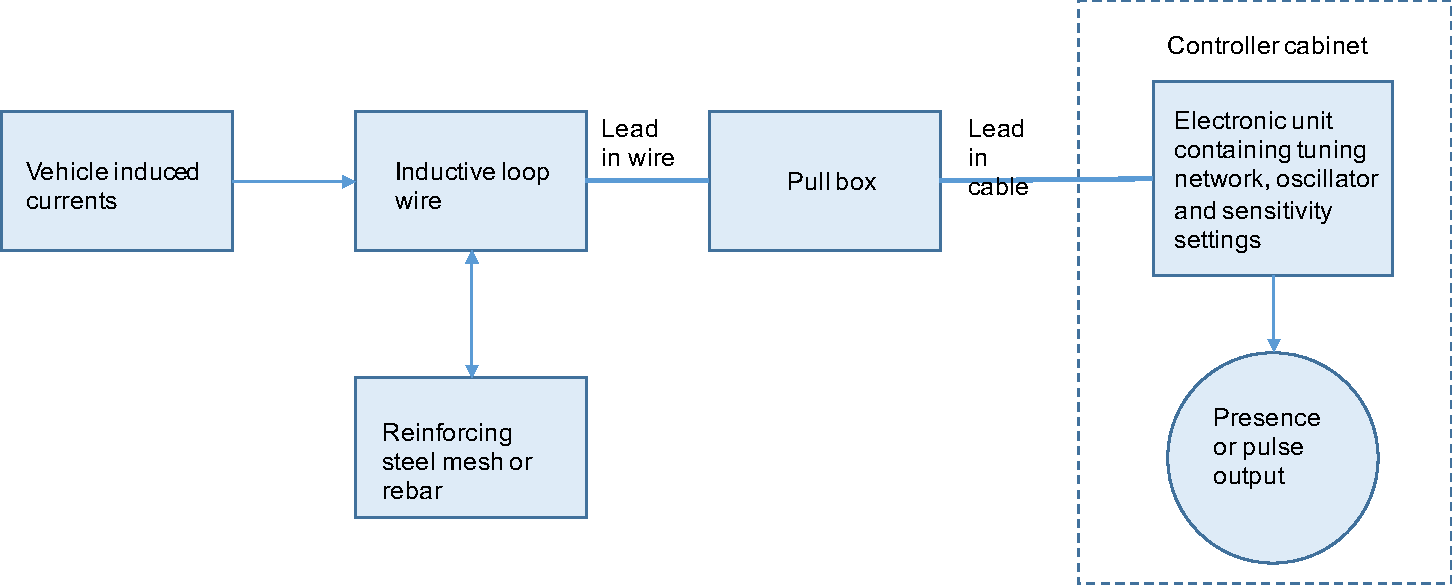
\includegraphics[width=0.7\textwidth,height=0.7\textheight,keepaspectratio]{Figures/loop-detector.pdf}
    \rule{35em}{0.5pt}
  \caption[A vehicle loop detector system]{An inductive loop detector system used for detecting the
  presence or passing of a vehicle. (Source - \textit{Traffic Detector Handbook: Third Edition—Volume I})}
  \label{fig:loopDetector}
\end{figure}

For this study a relatively large data set was used. This data set contains loop detector data collected
at several detection points in and around the Melbourne CBD. This dataset is a homogeneous set of
1084 road sections. A homogeneous section of the road is where the traffic flow normally remains unchanged
during the measured time period. The data was aggregated to a 15 minutes interval over a period
from 01/01/2008 to 25/07/2013, making a total 195168 observations.

\subsection{Measurement errors}
There are various factors that contribute to the measurement errors in traffic volume data. This can
at the vehicle loop detection system or at the traffic control center. The electronic unit that
detects the change in frequenct may not always be accrate leading to a false or missing reading.
We present the data casused by errors in two groups - missing data and false or unreliable data.

\subsubsection{Missing data}
Missing data occurs often in the case where either the loop detection system or the computer system
at the control center goes down. The missing period could vary between minutes to days depending on
the detection and resolution of the fault. Secondly the data could be missing for a certain location
or a set of locations.


As the data we acquired has zero value for missing data, it is difficult to say if that a zero value
is a result of missing data due to falut or a valid actual measurement. However we can aggregate the
data at a daily level, which then gives us a more better view of the missing data phenomena. Figure
\ref{fig:missing-days-count} shows the number of days for which no measurement was recorded for each
of the 1084 locations.

\begin{figure}[htbp]
  \centering
    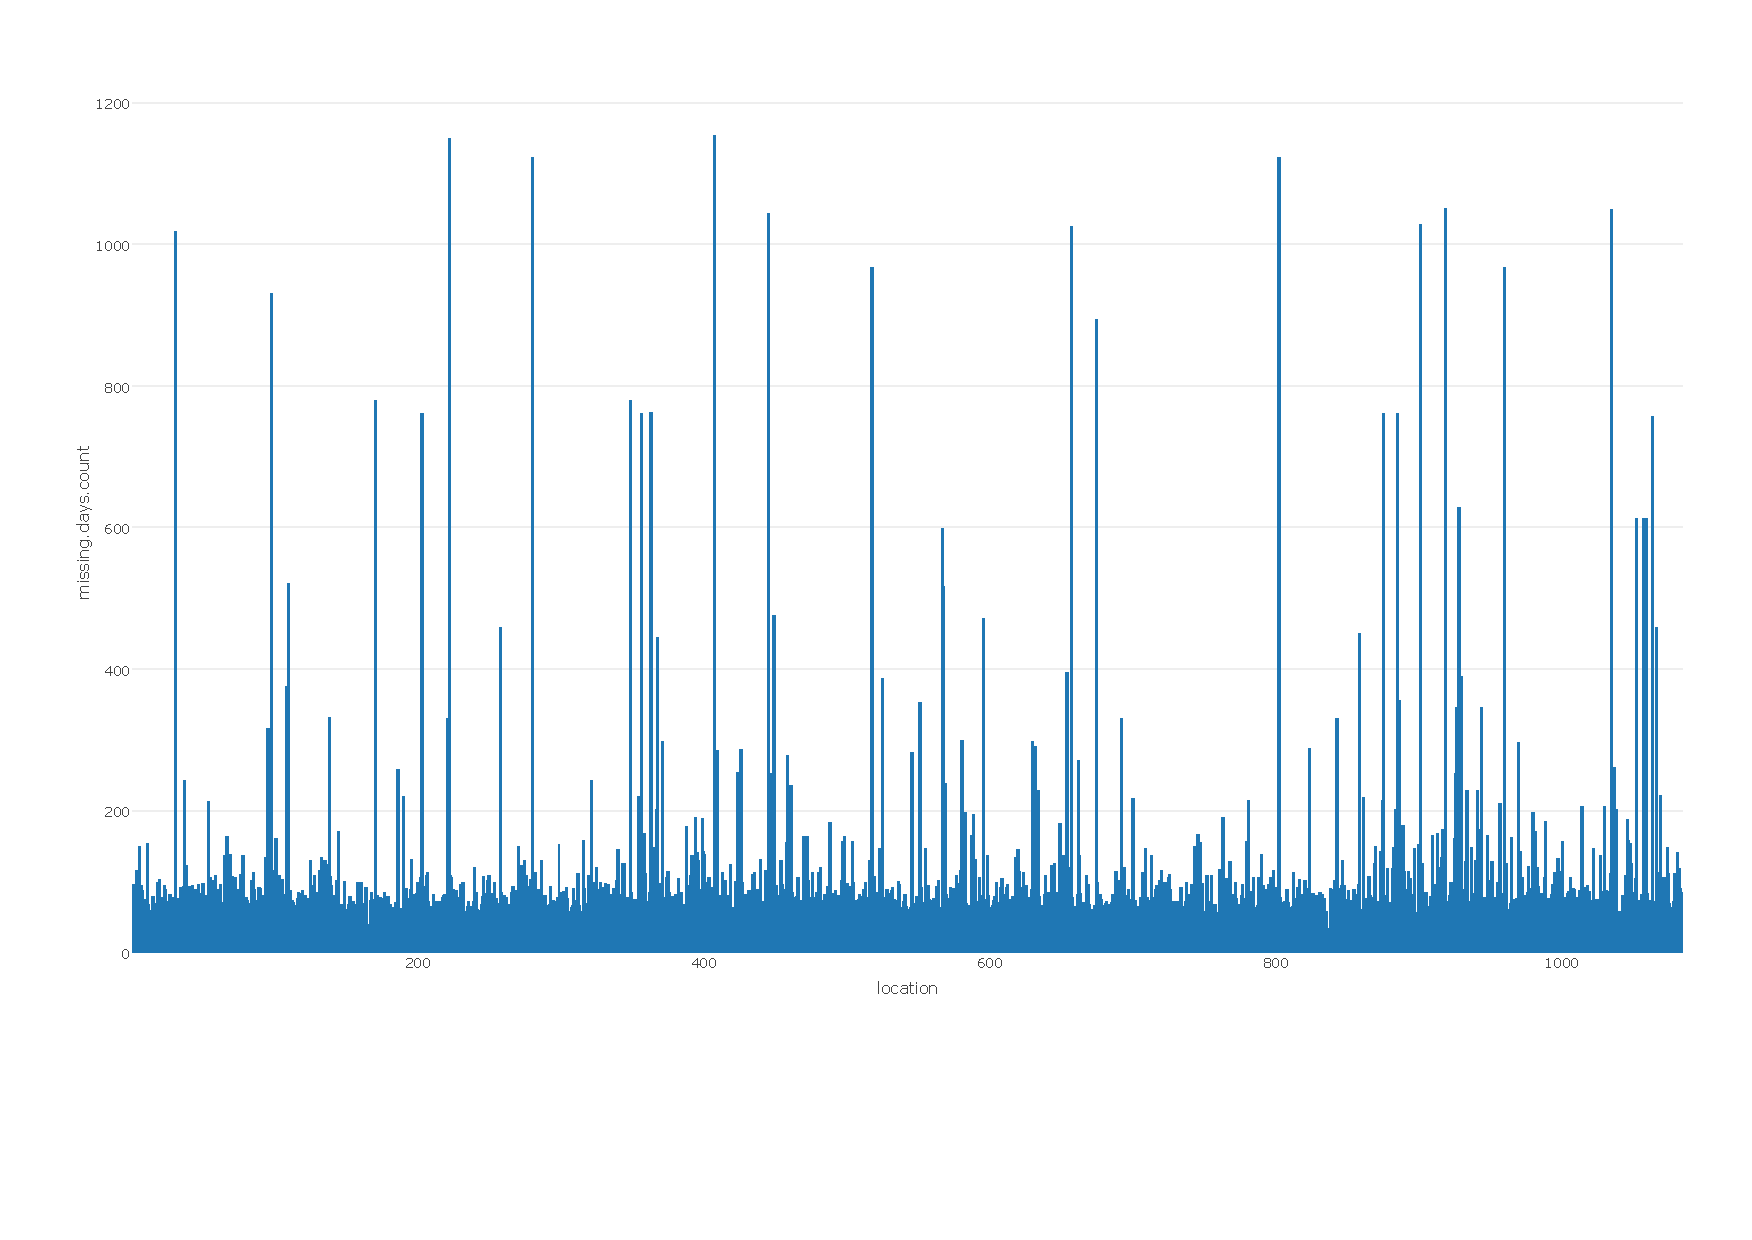
\includegraphics[width=\textwidth,height=\textheight,keepaspectratio]{Plots/missing-days-count.pdf}
    \rule{35em}{0.5pt}
  \caption[Missing data]{Missing data - number of days when no measurement was recorded at each of
  the 1084 locations in our data. The locations are shown as index numbers.}
  \label{fig:missing-days-count}
\end{figure}

We can see the number of missing data it is quite significant and it can largely affect the model for
short term traffic prediction. There are several imputation strategies that are usually used in practice
to deal with missing data in traffic data. One of the methods is known as historical imputation. In this
method previously collected data at simliar time interval at the same location is used to fill in the missing
value. The distance in time is often selected as minimum as possible. A variation of this is another
simple approach that takes an average of past few recorded observations and uses that to fill in
the missing data. A second method that is used is splie/linear regression regression that interpolates
the missing value from neighbourhood data points.

\subsubsection{Unreliable data}
Unreleable data is observed when the measurements recorded by the loop detectors show unreasonably
large deviations. This is due to some fault in the loop detector system. These are obvious to the
naked eyes when looking at the plot of the measurements but hard to detect automatically. Such errors
are usually detected during preprocessing by setting a maximum value that a meaurement can have. The
maximum value can be obtained using the frequency distributions of the measurements.

\section{Analysis of the traffic volume data}

% location lat-lng (start -37.8099,144.9913, end
In this section, we present some analysis on the traffic volume data as mentioned earlier in previous
section. For this we chose the location with least number of missing data. This location is with HF
number 16913 (Victoria street) which is located on the north-east of Melbourne CBD as shown in the
figure \ref{fig:ExperimentRegion} annotated in red.

\begin{figure}[htbp]
  \centering
    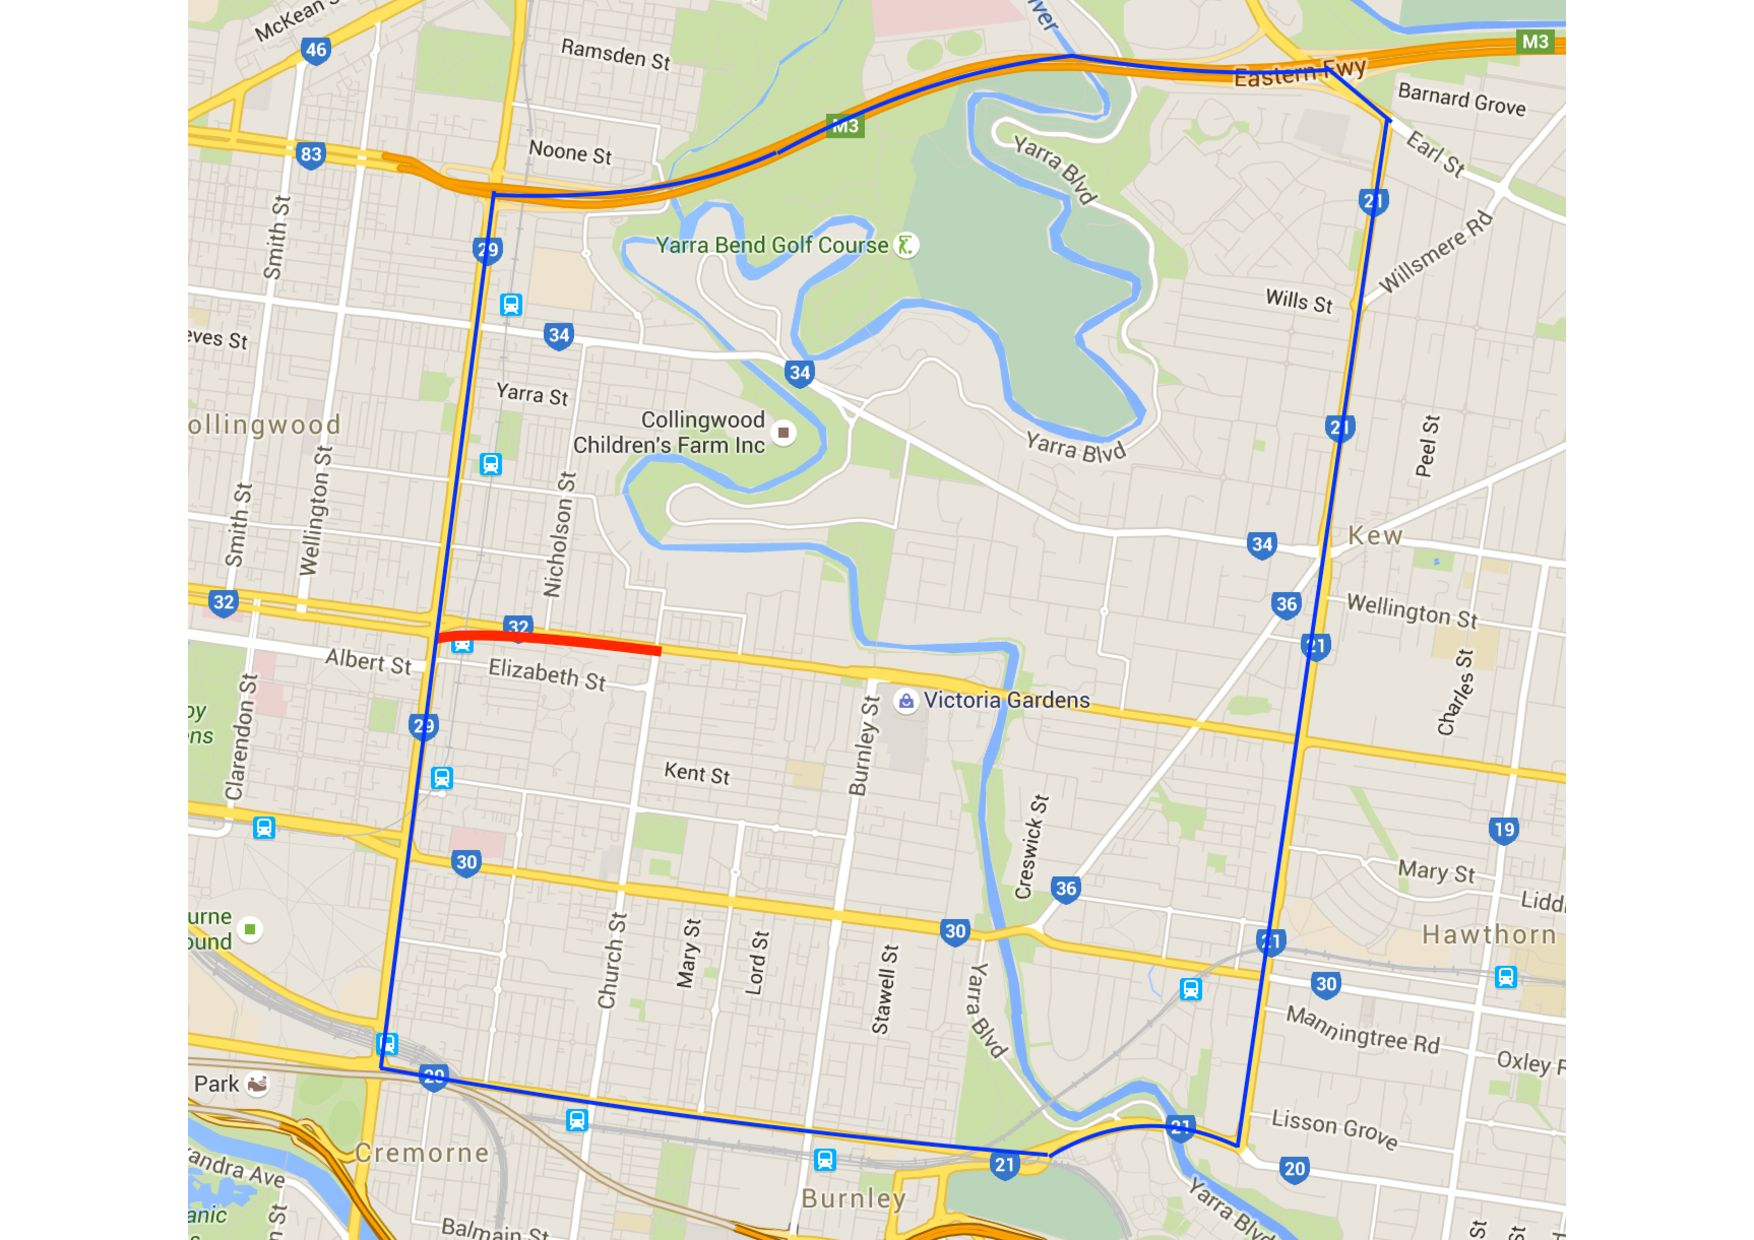
\includegraphics[width=0.7\textwidth,height=0.7\textheight,keepaspectratio]{Figures/experiment-region.pdf}
    \rule{35em}{0.5pt}
  \caption[Experiment traffic region]{The traffic region used in this experiment. The boundary is
   dentoed by the red line.}
  \label{fig:ExperimentRegion}
\end{figure}


\subsection{Syatmatic variations}

\subsubsection{Daily variations}
First we would like to see how traffic volume changes over time during a day and over the days during
a week. Figure \ref{fig:TypicalDay} shows how traffic volume on a random day looks like.

\begin{figure}[htbp]
  \centering
    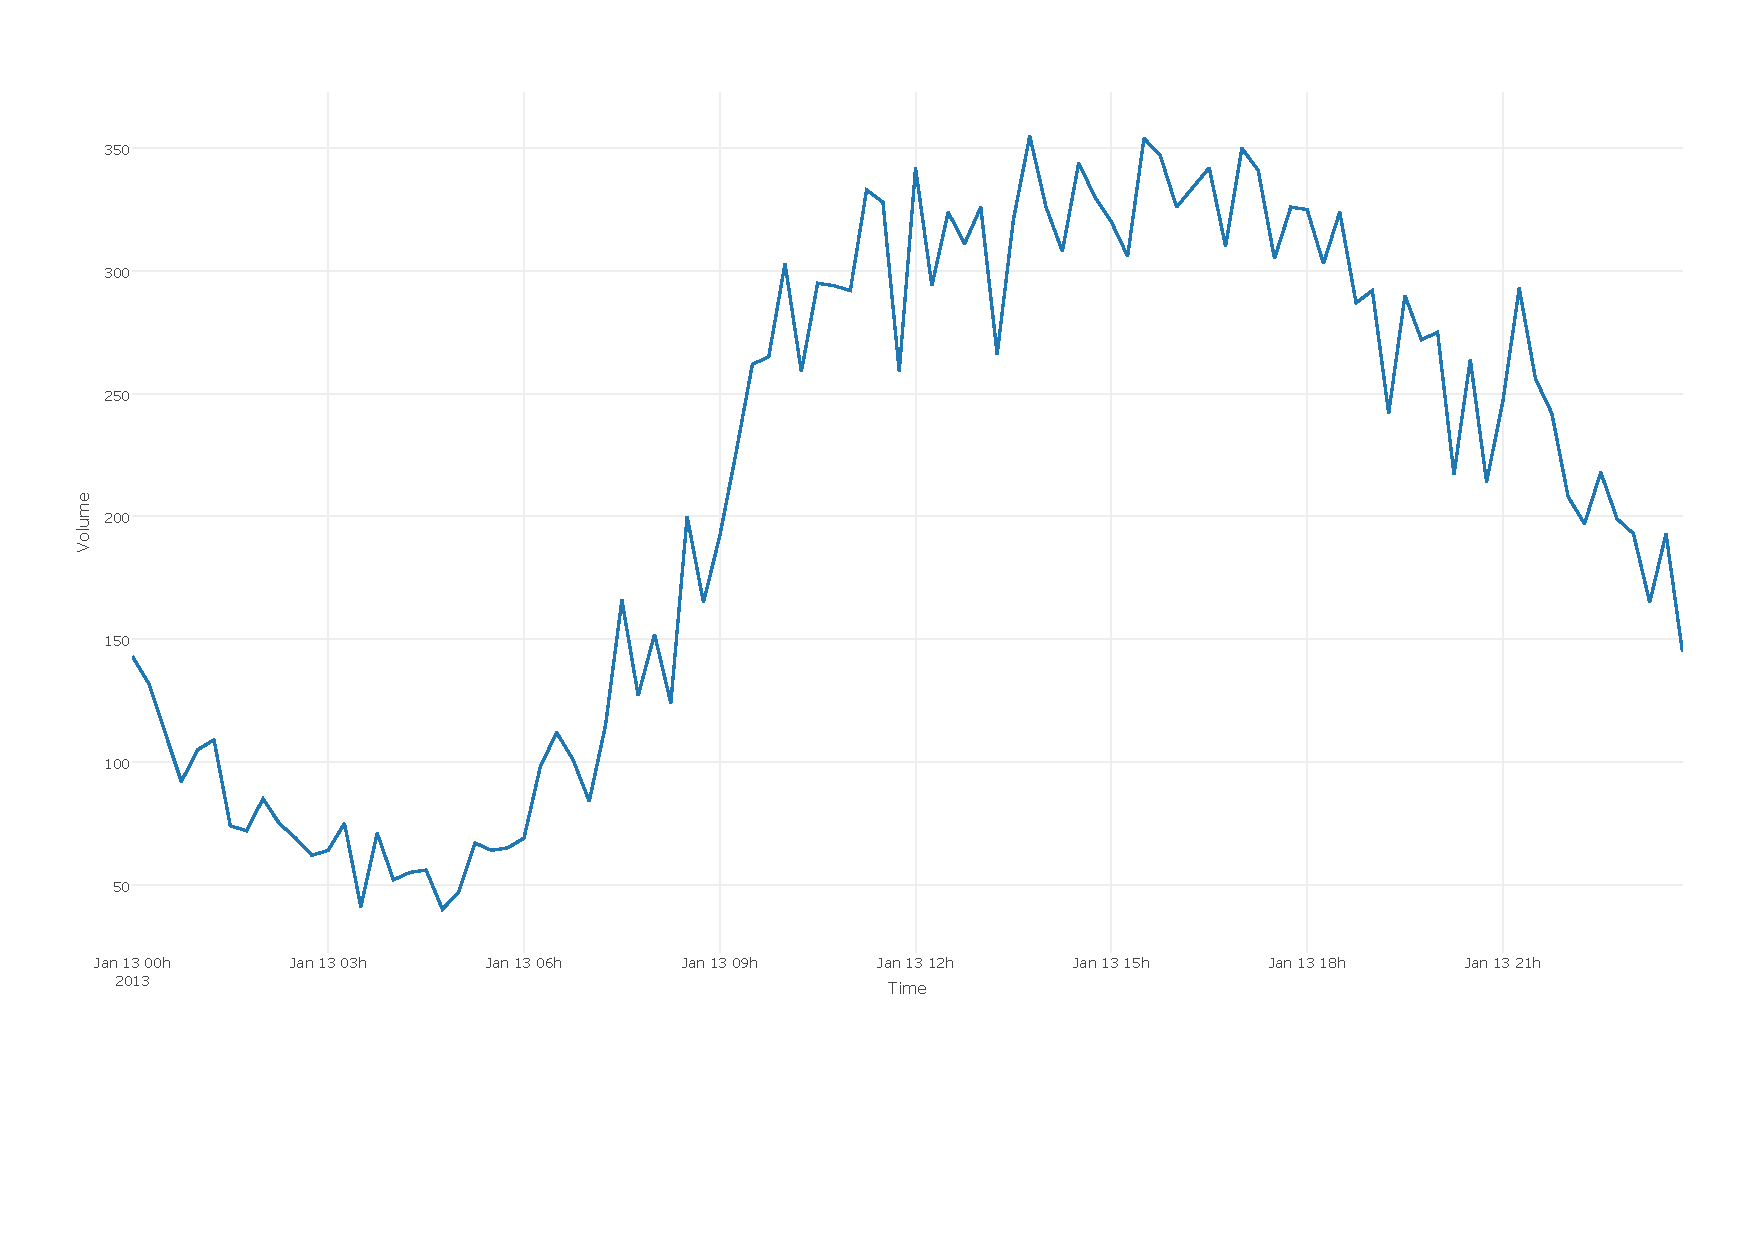
\includegraphics[width=0.7\textwidth,height=0.7\textheight,keepaspectratio]{Plots/typical-day.pdf}
    \rule{35em}{0.5pt}
  \caption[A typical day traffic flow]{Variations in traffic flow on a typical day.}
  \label{fig:TypicalDay}
\end{figure}

To find out in overall how traffic volume looks like on each day of the week, we have grouped the
traffic data into seven classes for each day of the week. Then for each class we grouped the data
in it by time and took an average. In figure \ref{TypicalDayTraffic} We plot the results.


\begin{figure}[h]
    \centering
    \subfloat[Monday][Monday]{
    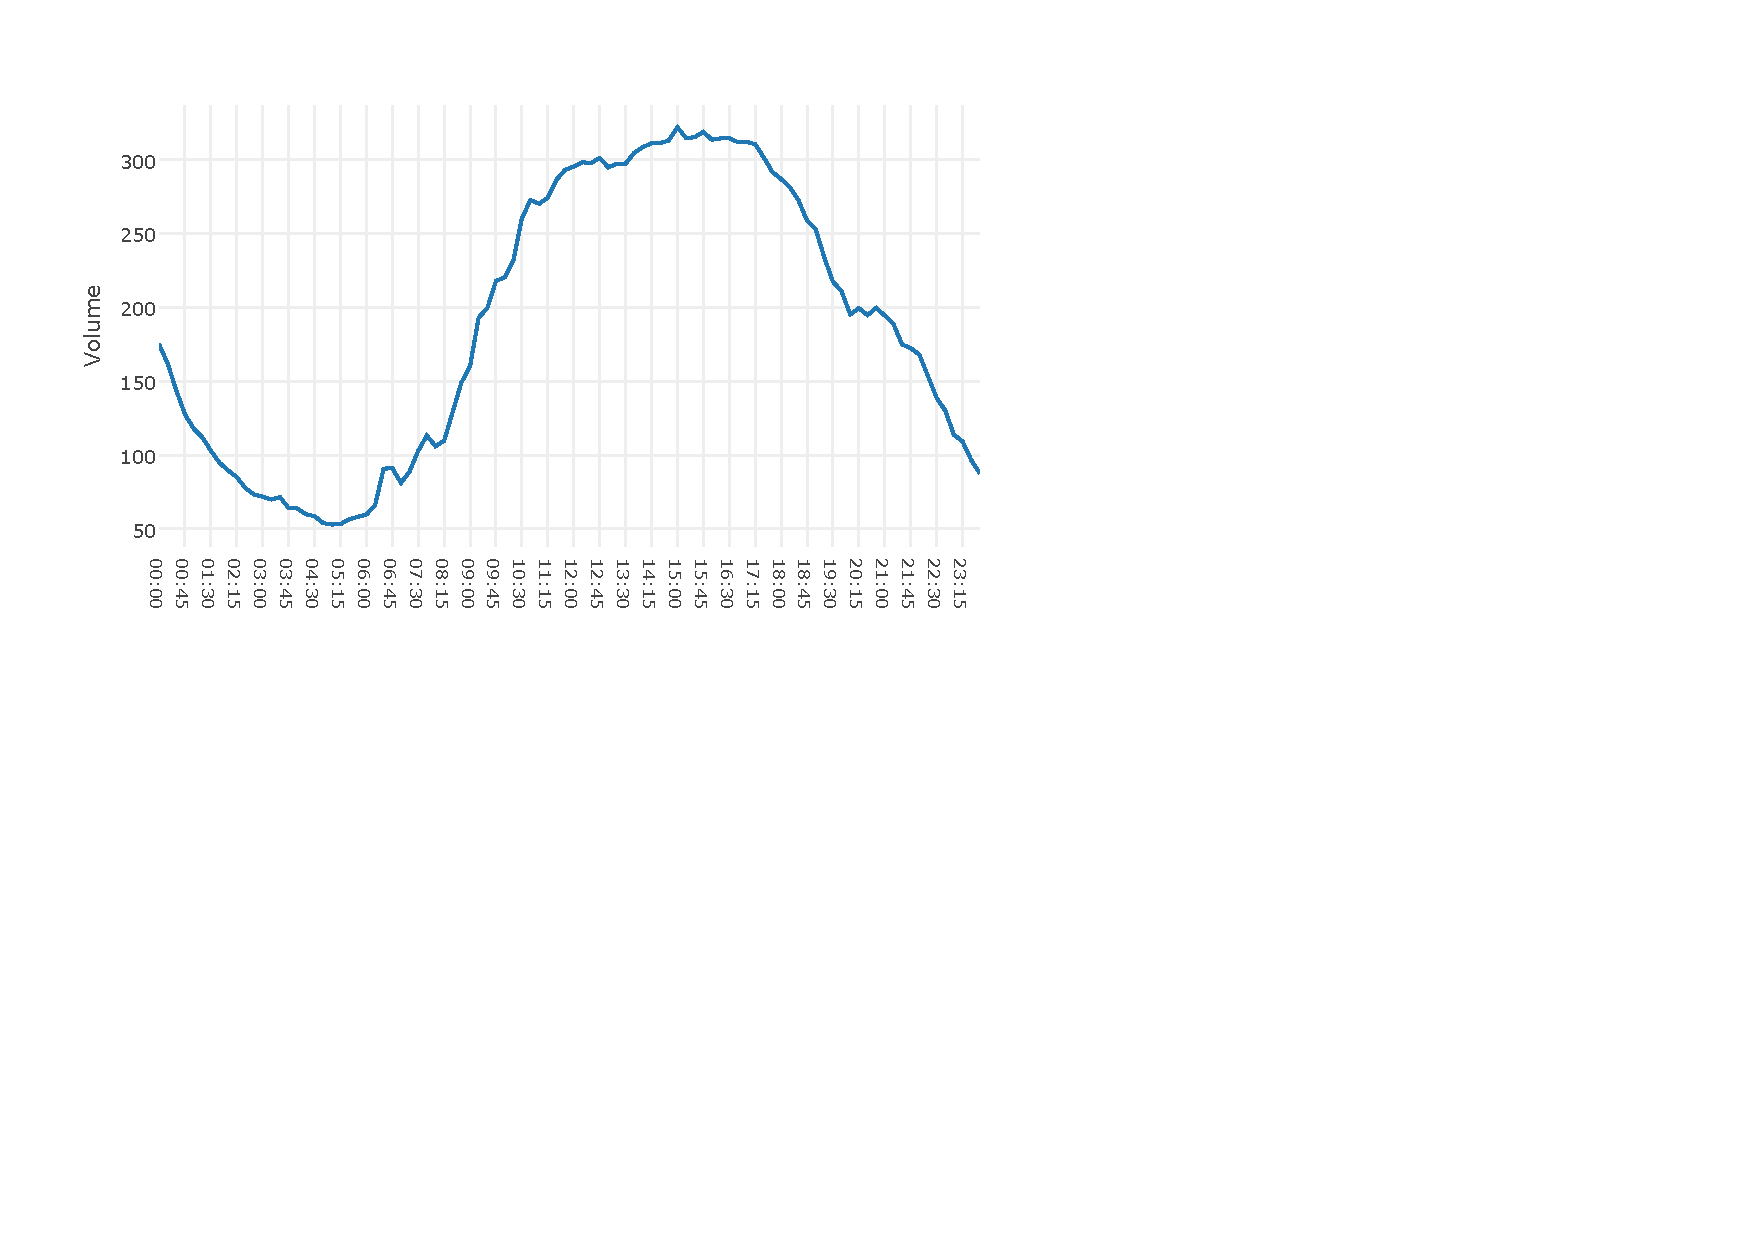
\includegraphics[width=0.4\textwidth]{Plots/typical-monday.pdf}
    \label{fig:typicalMonday}}
    \qquad
    \subfloat[Tuesday][Tuesday]{
    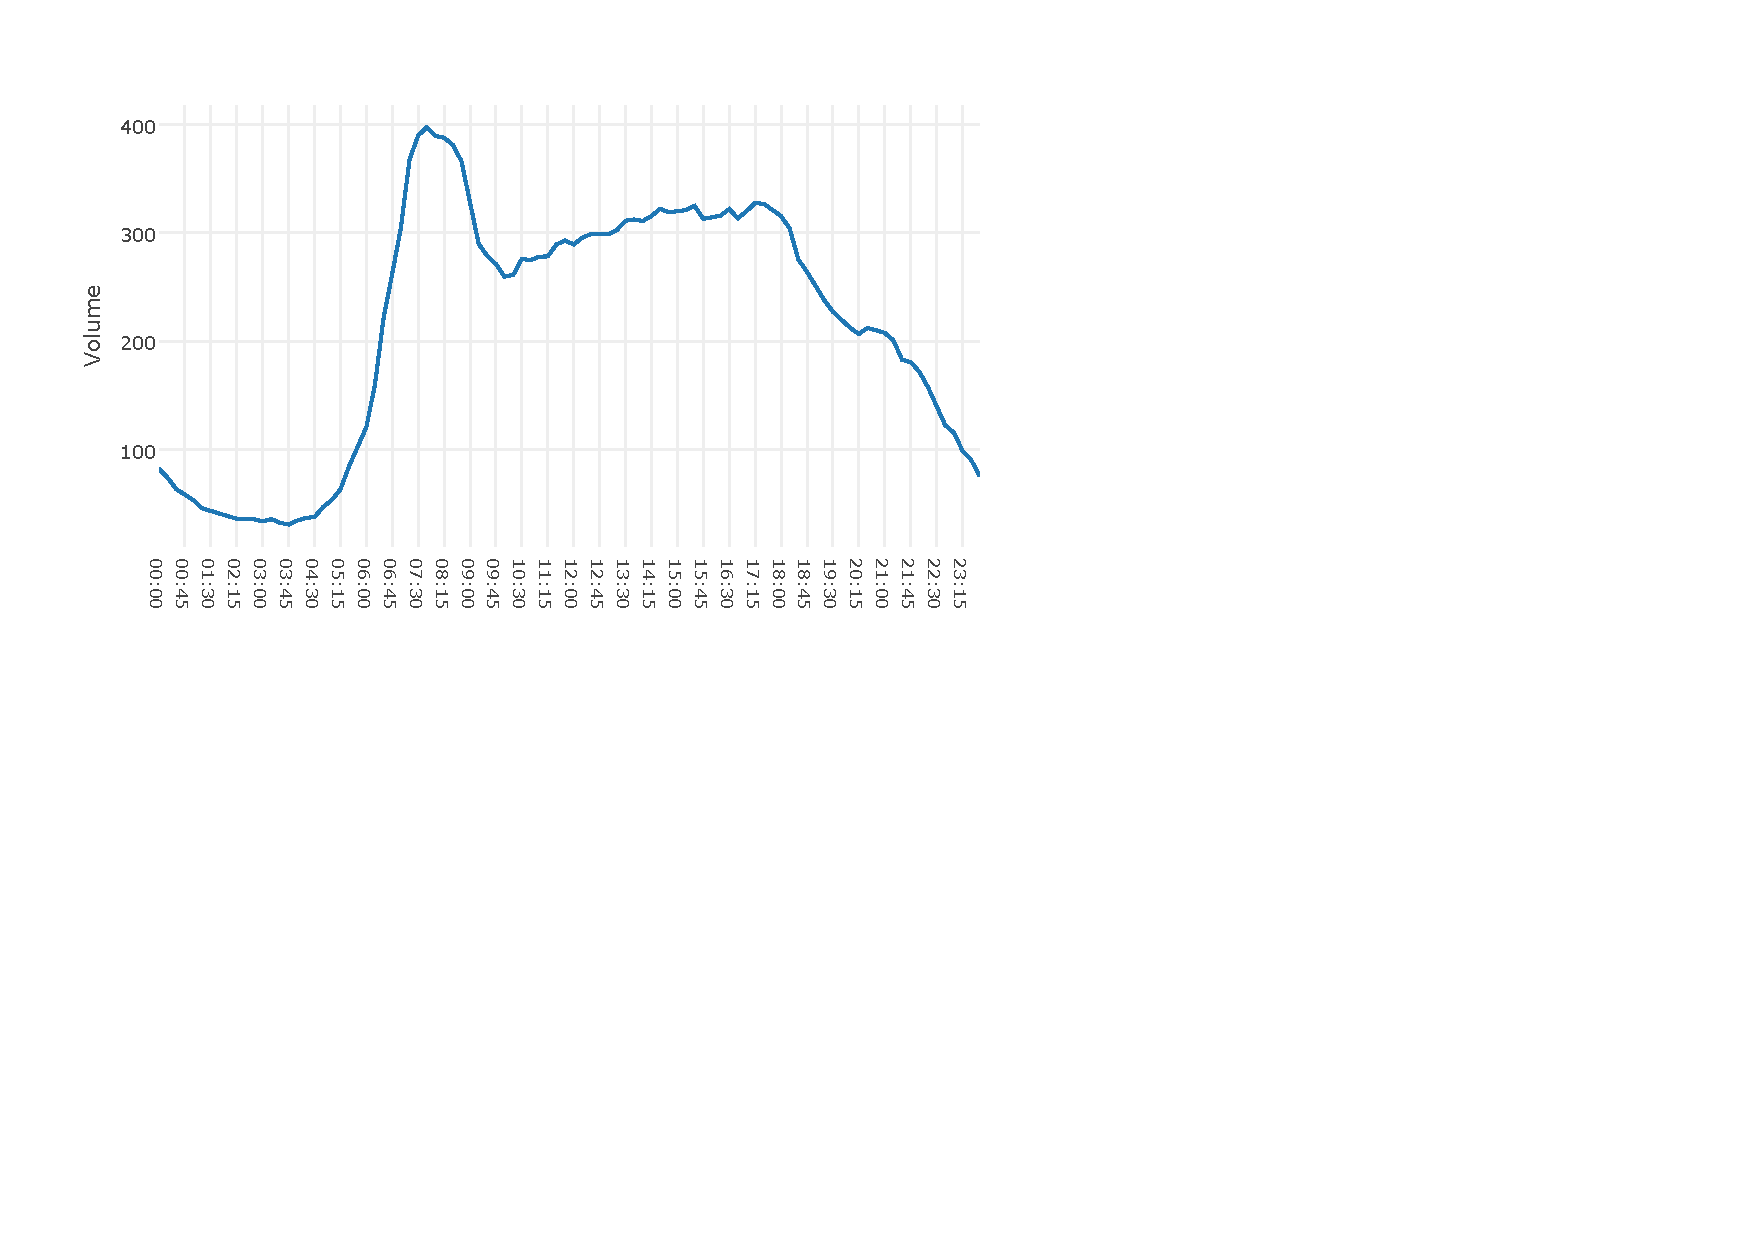
\includegraphics[width=0.4\textwidth]{Plots/typical-tuesday.pdf}
    \label{fig:typicalTuesday}}

    \subfloat[Wednesday][Wednesday]{
    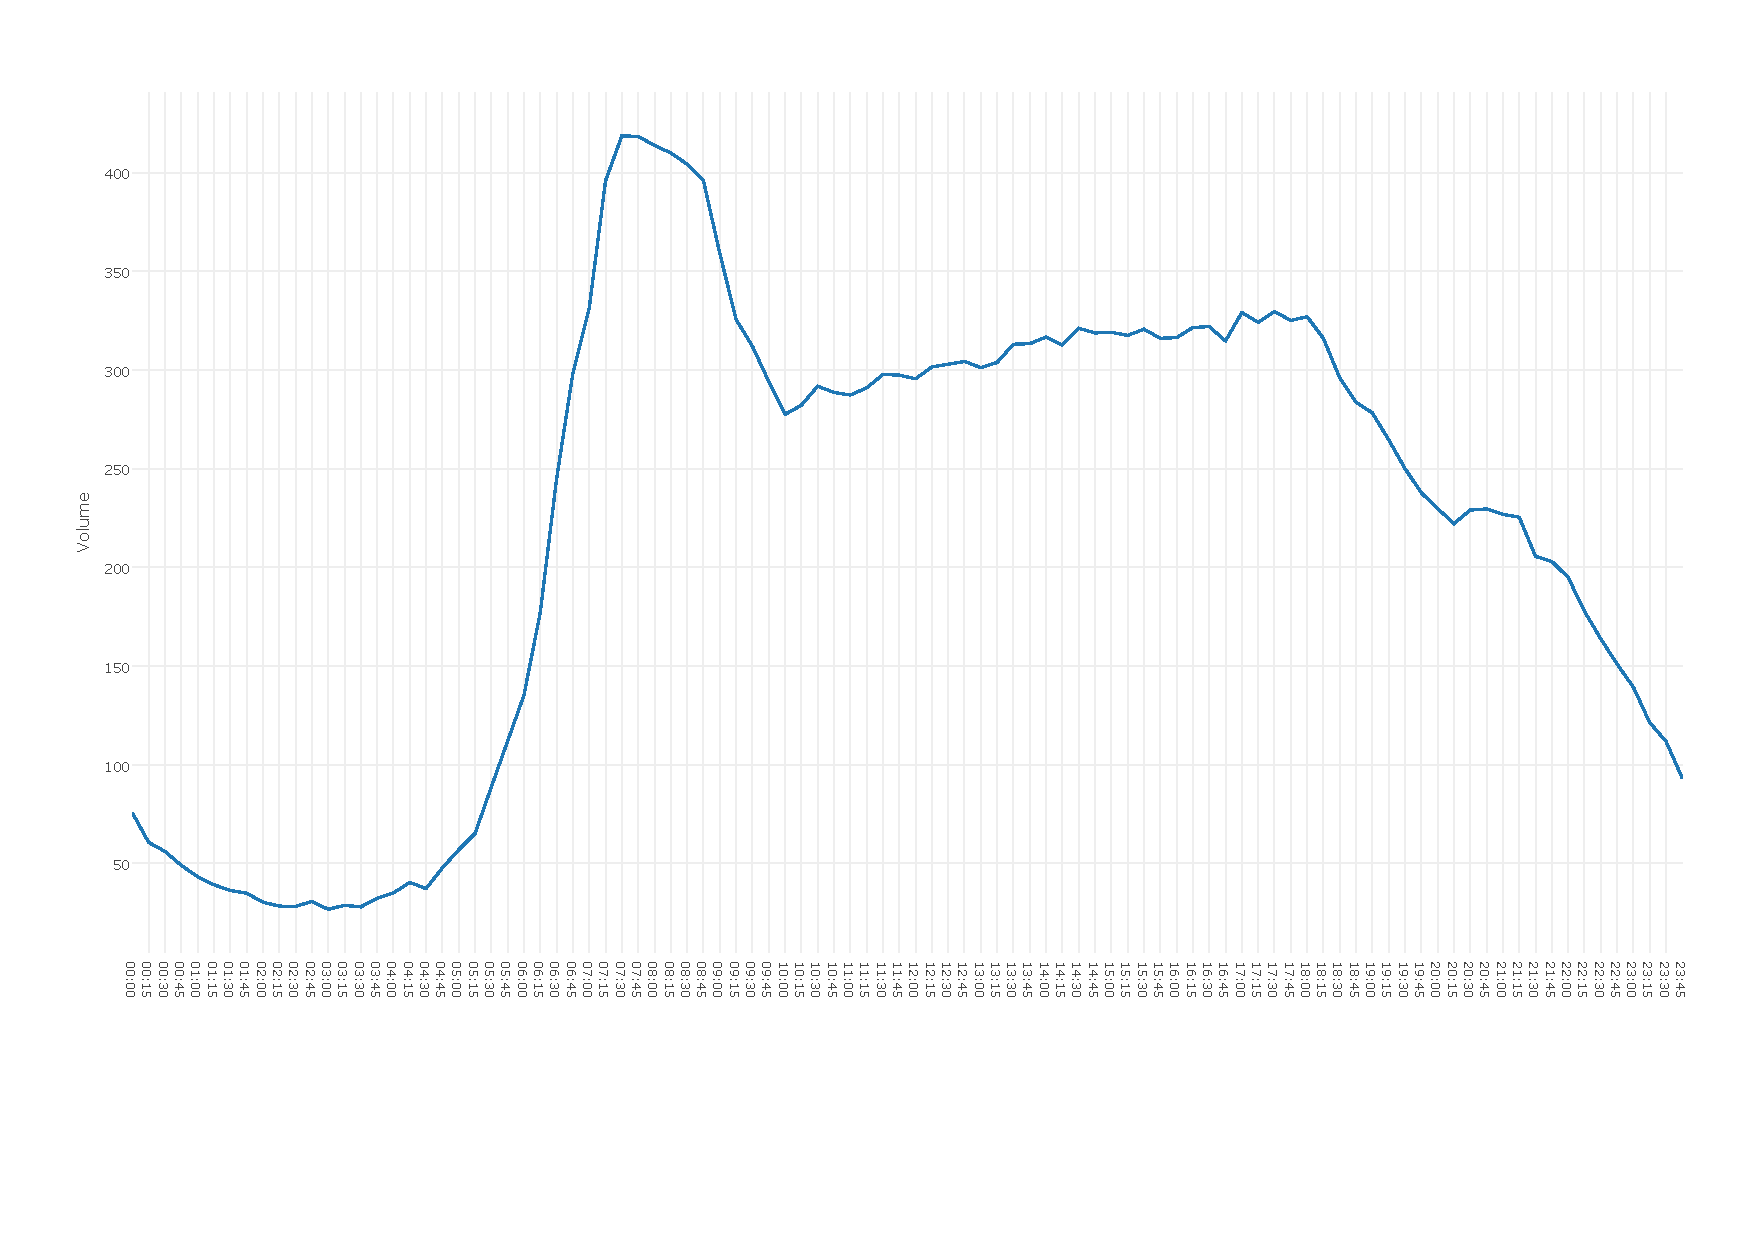
\includegraphics[width=0.4\textwidth]{Plots/typical-wednesday.pdf}
    \label{fig:typicalWednesday}}
    \qquad
    \subfloat[Thursday][Thursday]{
    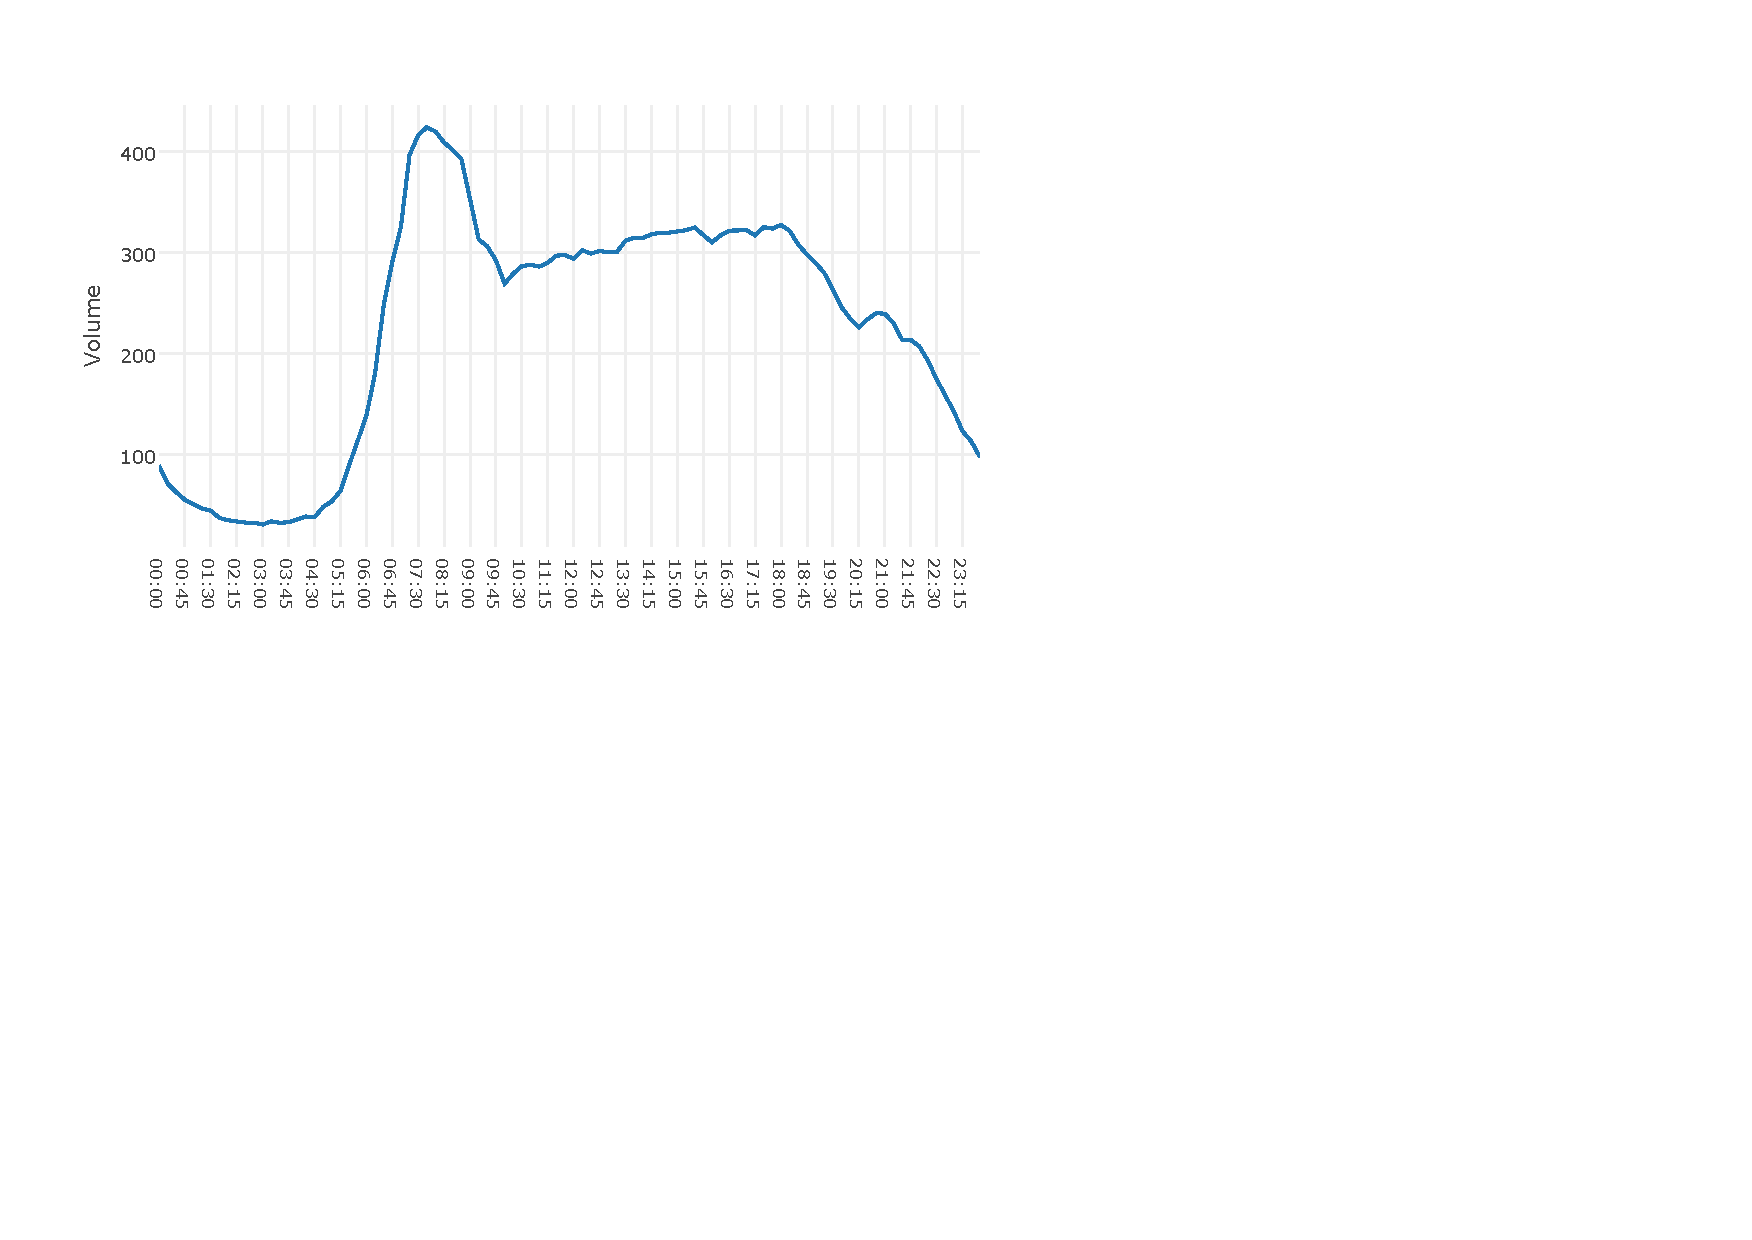
\includegraphics[width=0.4\textwidth]{Plots/typical-thursday.pdf}
    \label{fig:typicalThursday}}

    \subfloat[Friday][Friday]{
    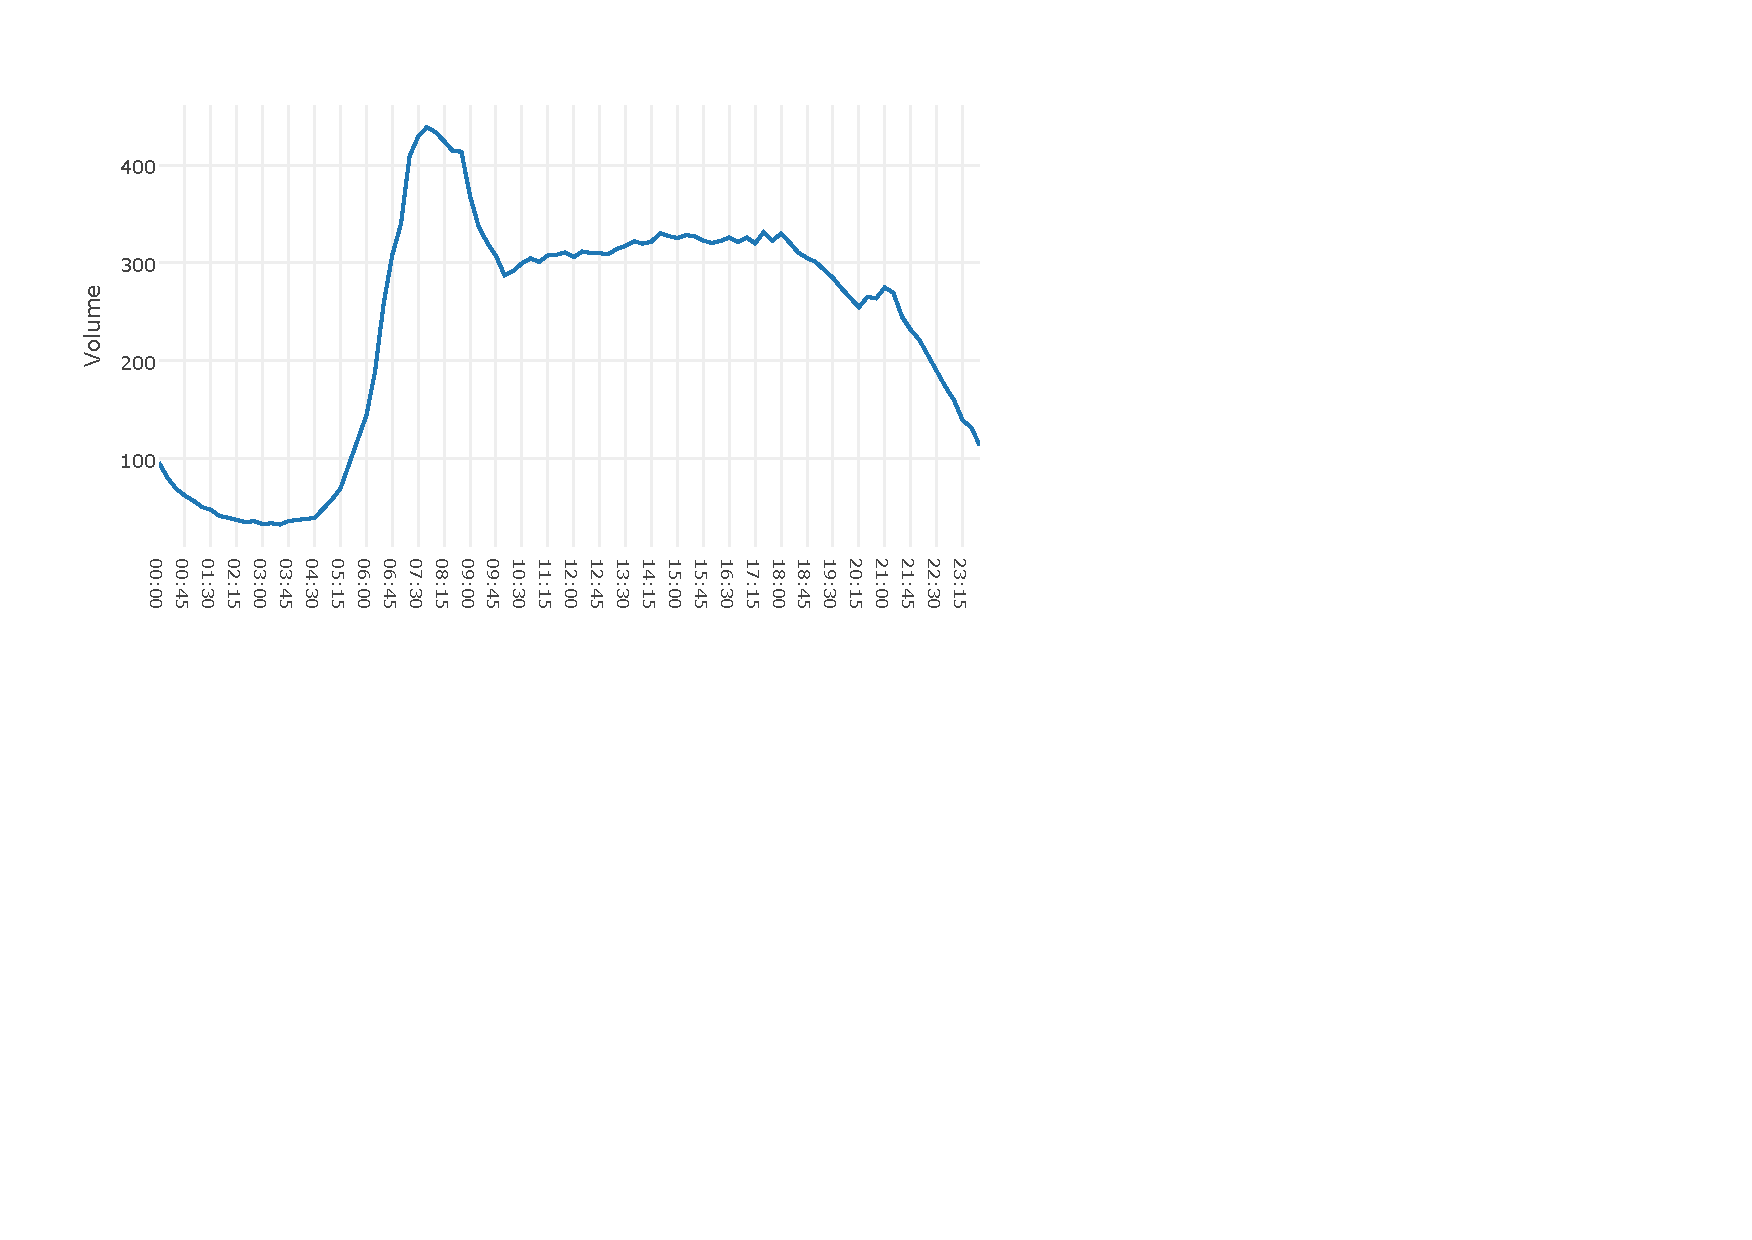
\includegraphics[width=0.4\textwidth]{Plots/typical-friday.pdf}
    \label{fig:typicalFriday}}
    \qquad
    \subfloat[Saturday][Saturday]{
    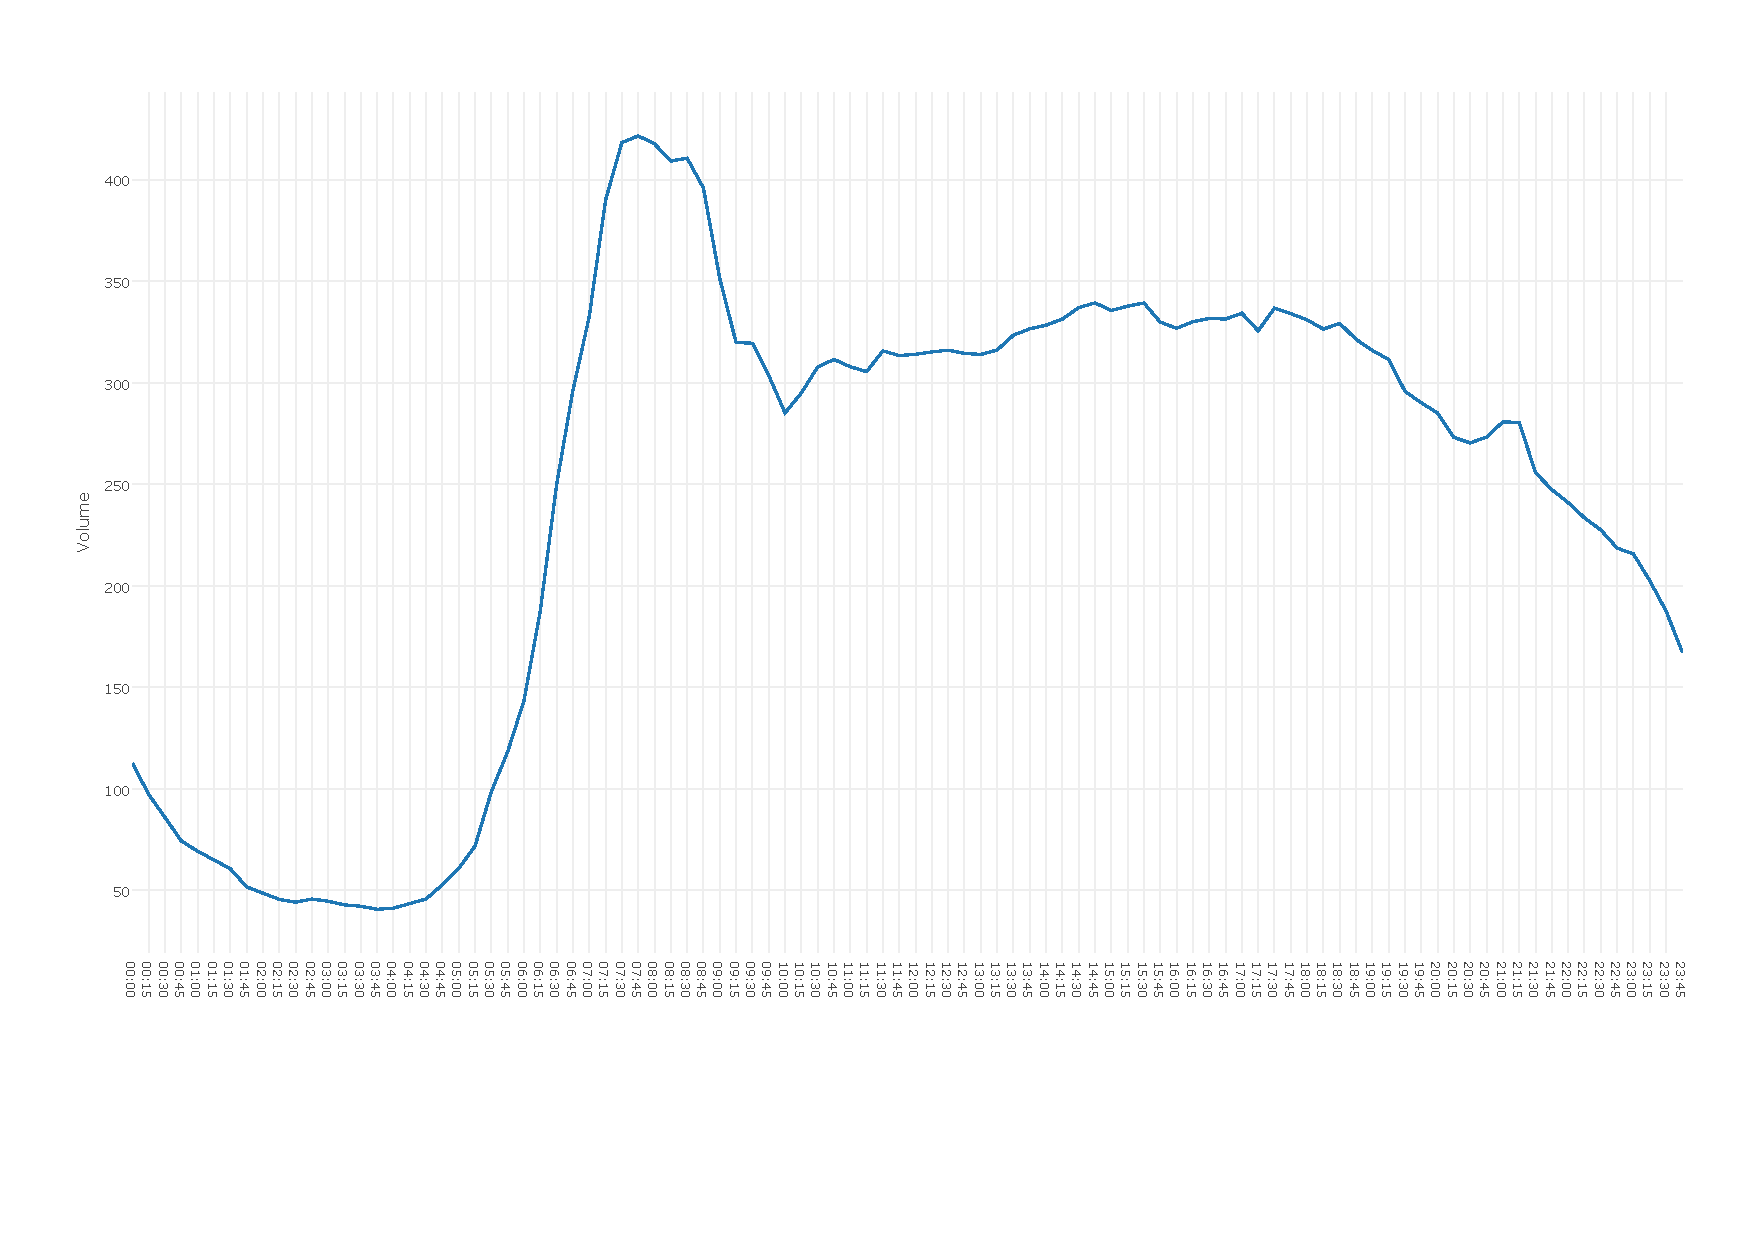
\includegraphics[width=0.4\textwidth]{Plots/typical-saturday.pdf}
    \label{fig:typicalSaturday}}

    \subfloat[Sunday][Sunday]{
    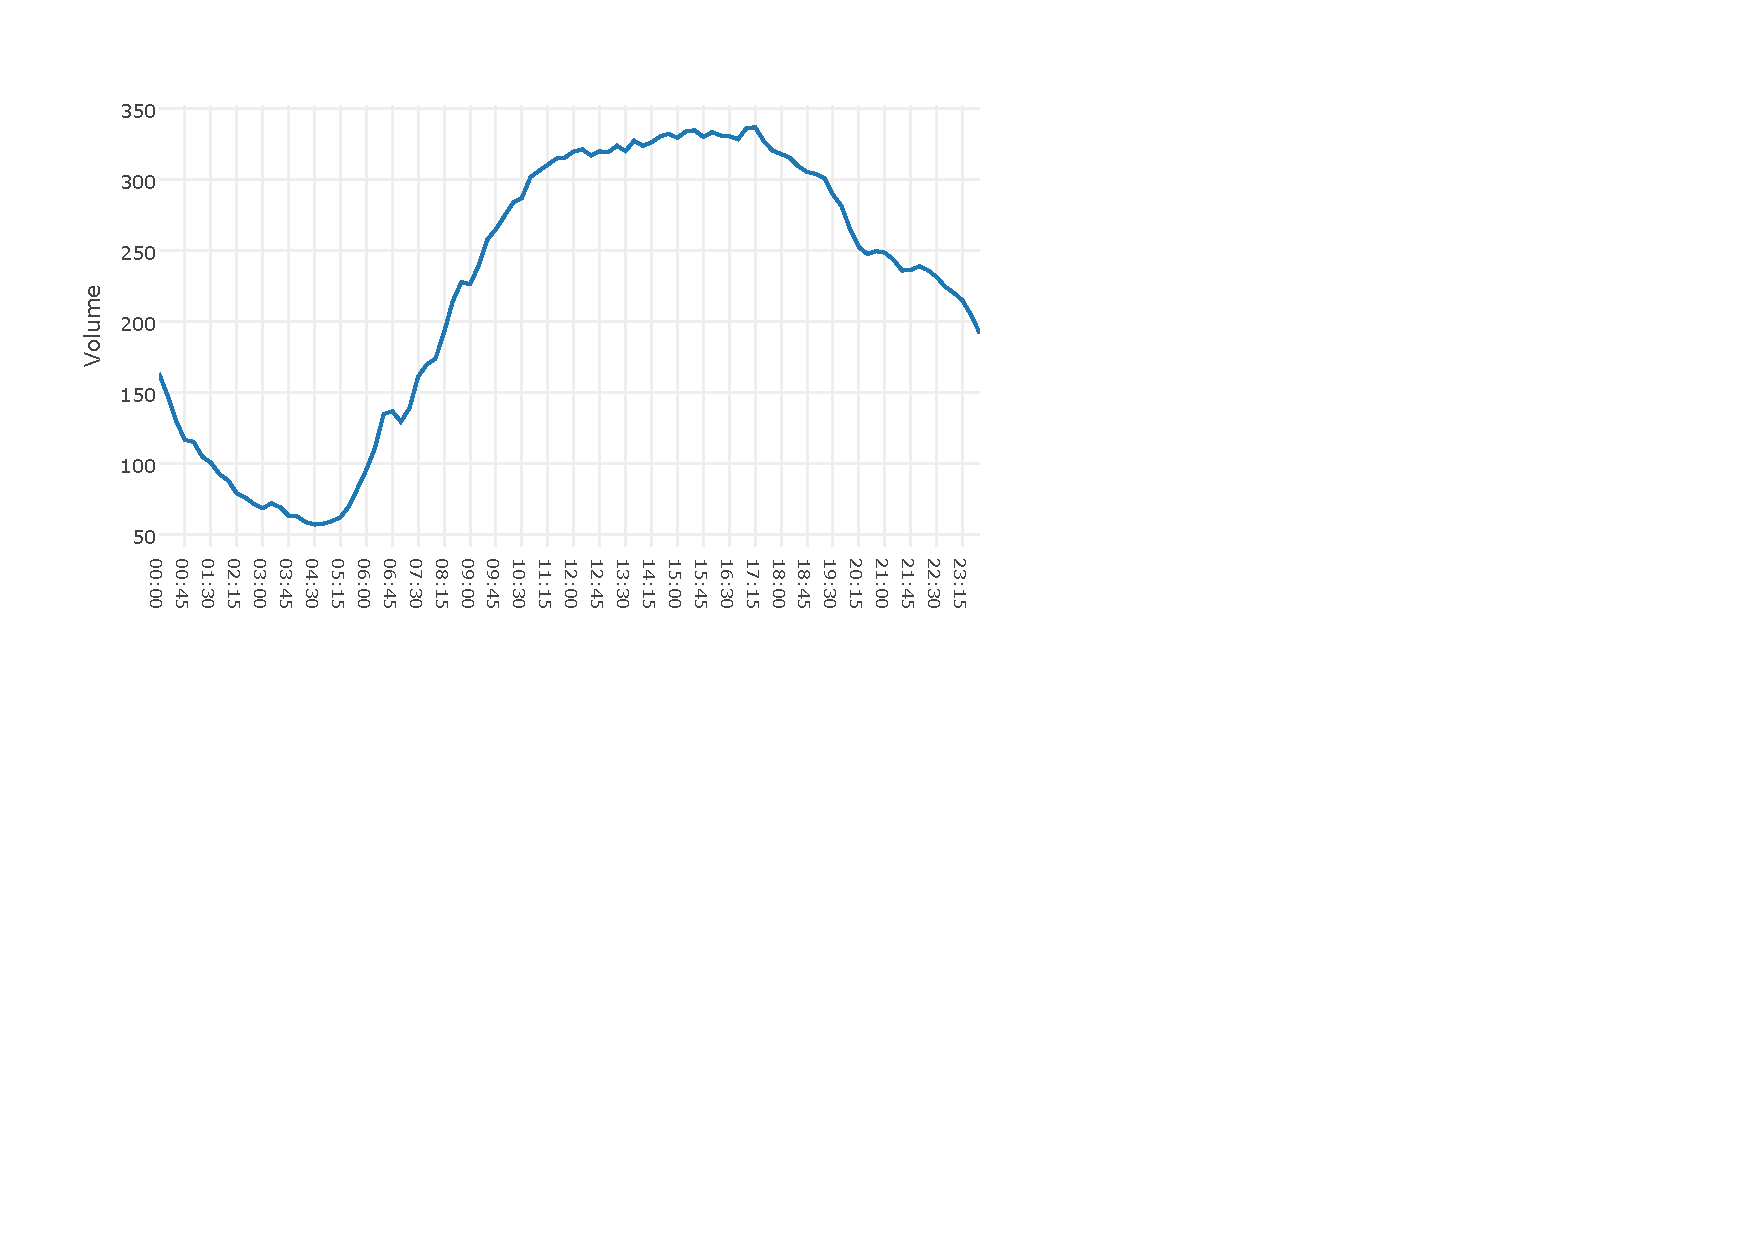
\includegraphics[width=0.4\textwidth]{Plots/typical-sunday.pdf}
    \label{fig:typicalSunday}}

    \caption[Traffic grouped by every day of the week]{Traffic grouped by every day of the week.}
    \label{fig:TypicalDayTraffic}
\end{figure}

\subsubsection{Seasonal variations}

Weekly, monthly and annual variations

\begin{figure}[h]
   \centering
    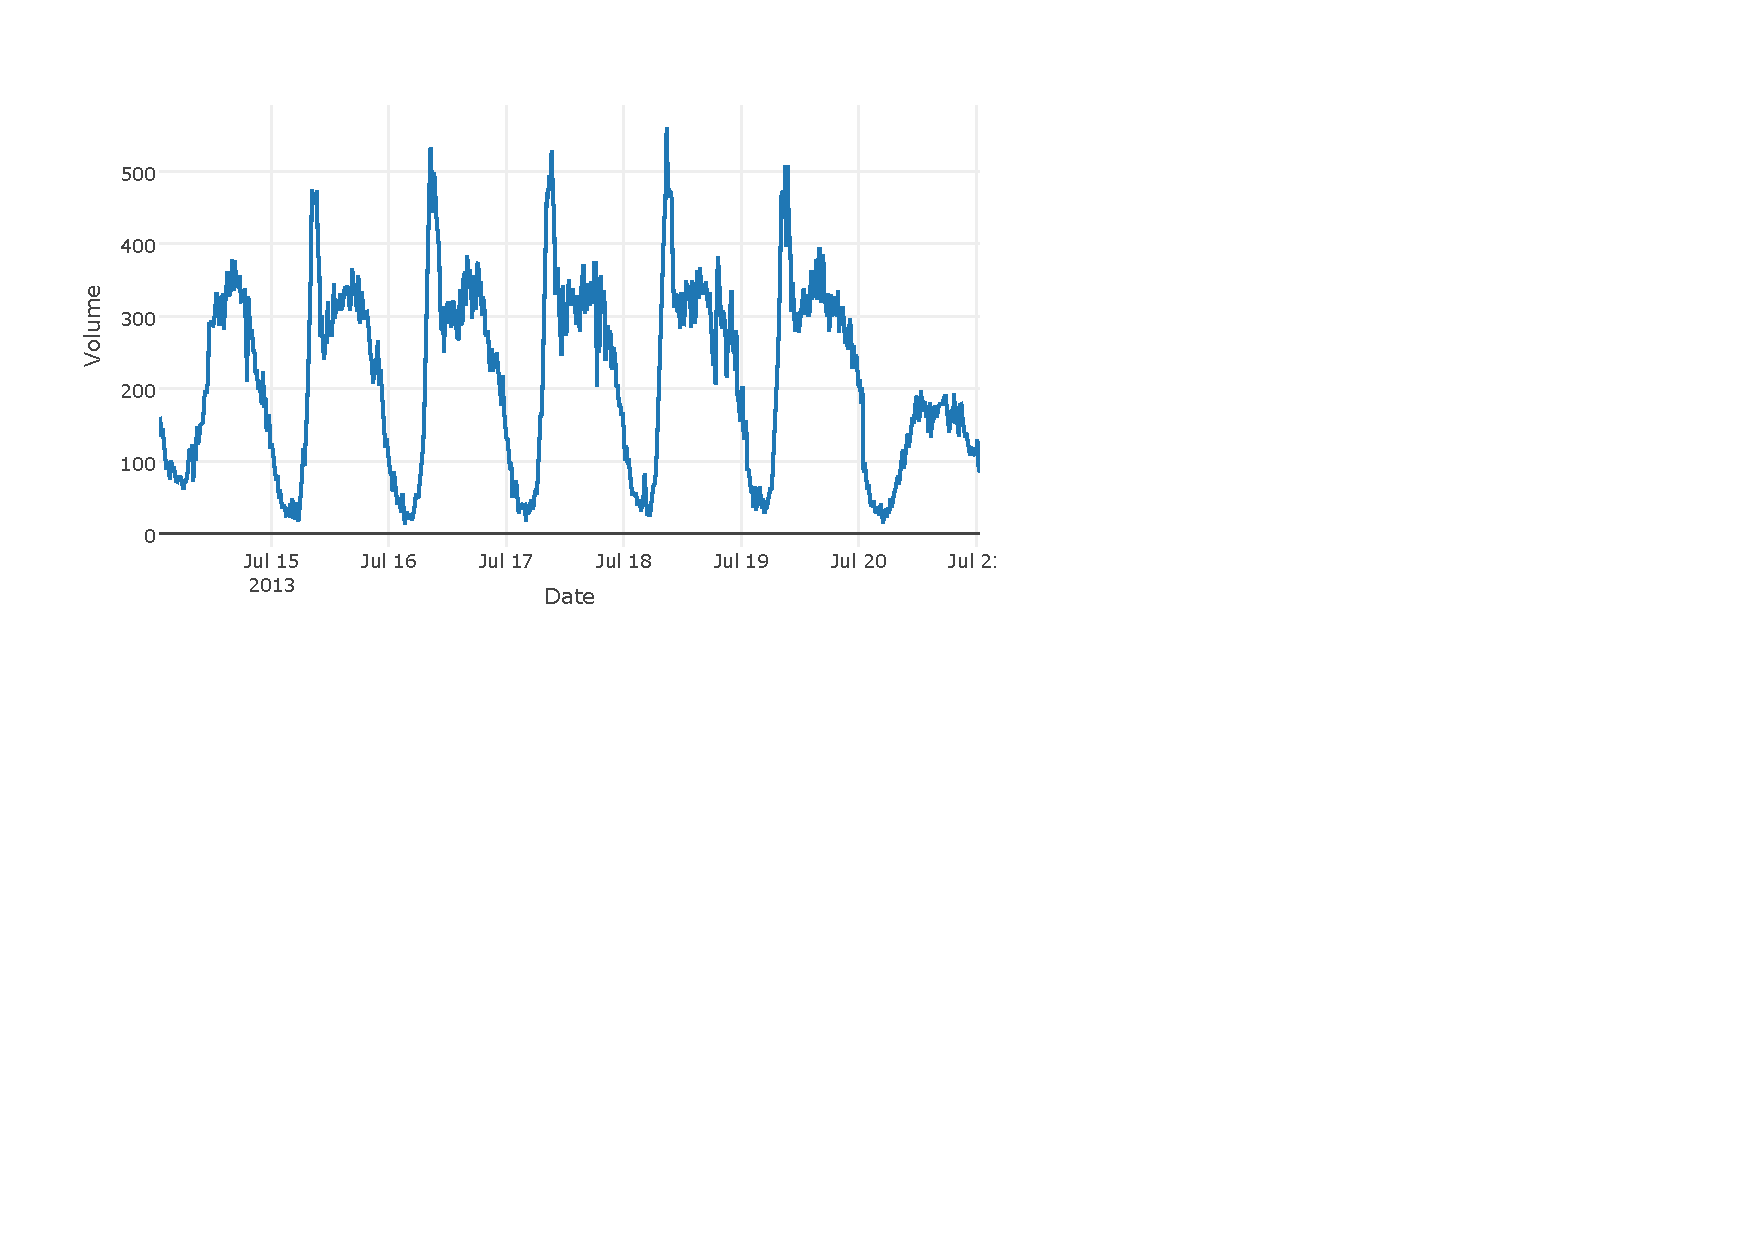
\includegraphics[width=0.7\textwidth,height=0.7\textheight,keepaspectratio]{Plots/typical-week.pdf}
    \rule{35em}{0.5pt}
  \caption[A typical week traffic flow]{Variations in traffic flow on a typical week.}
  \label{fig:TypicalWeek}
\end{figure}

\subsubsection{Outliers}

Variations caused by public events or non-recurrent events such as accidents, road work etc.

In fig \ref{fig:Holidays}, we can see the variation in traffic flow on public holidays.

\begin{figure}[h]
    \centering
    \subfloat[Mondays][Mondays]{
    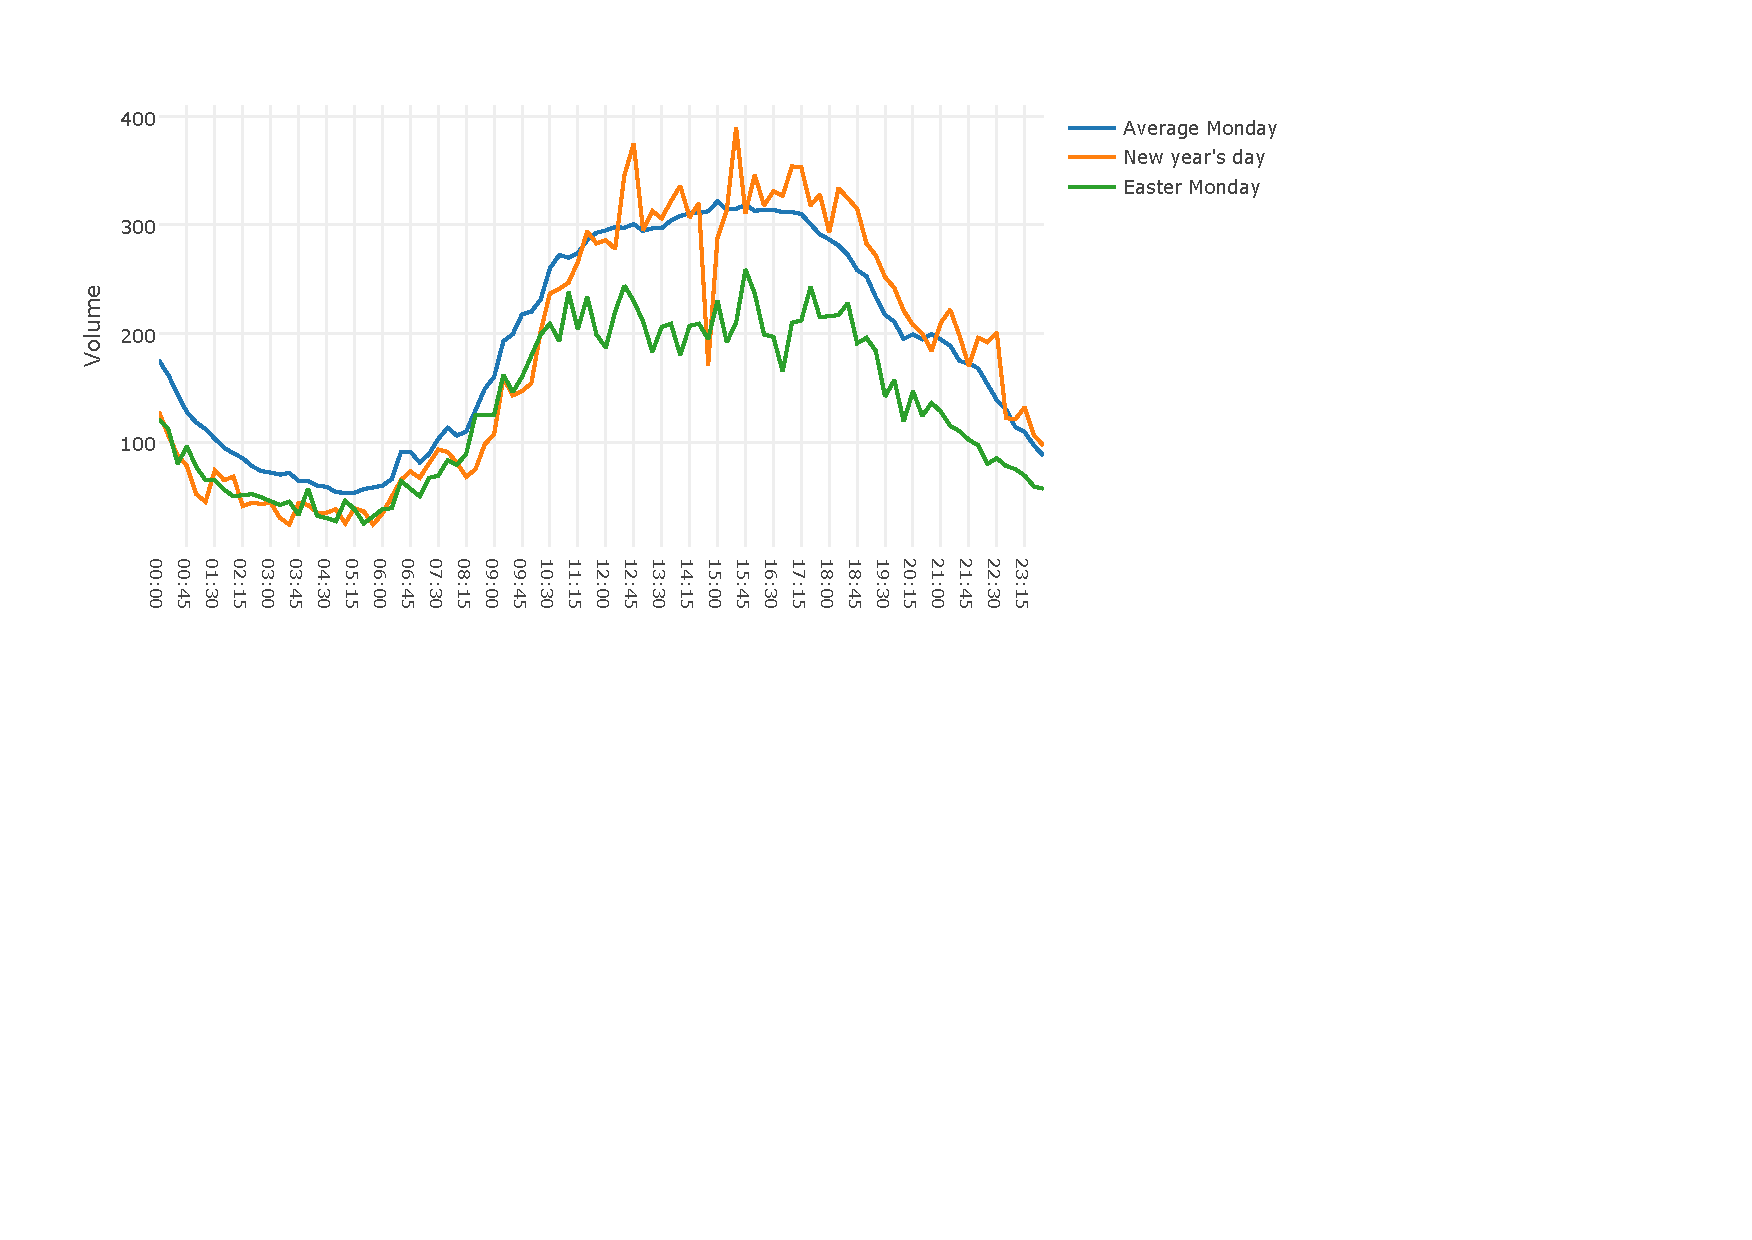
\includegraphics[width=0.4\textwidth]{Plots/holiday-mondays.pdf}
    \label{fig:HolidayMondays}}
    \qquad
    \subfloat[Tuesdays][Tuesdays]{
    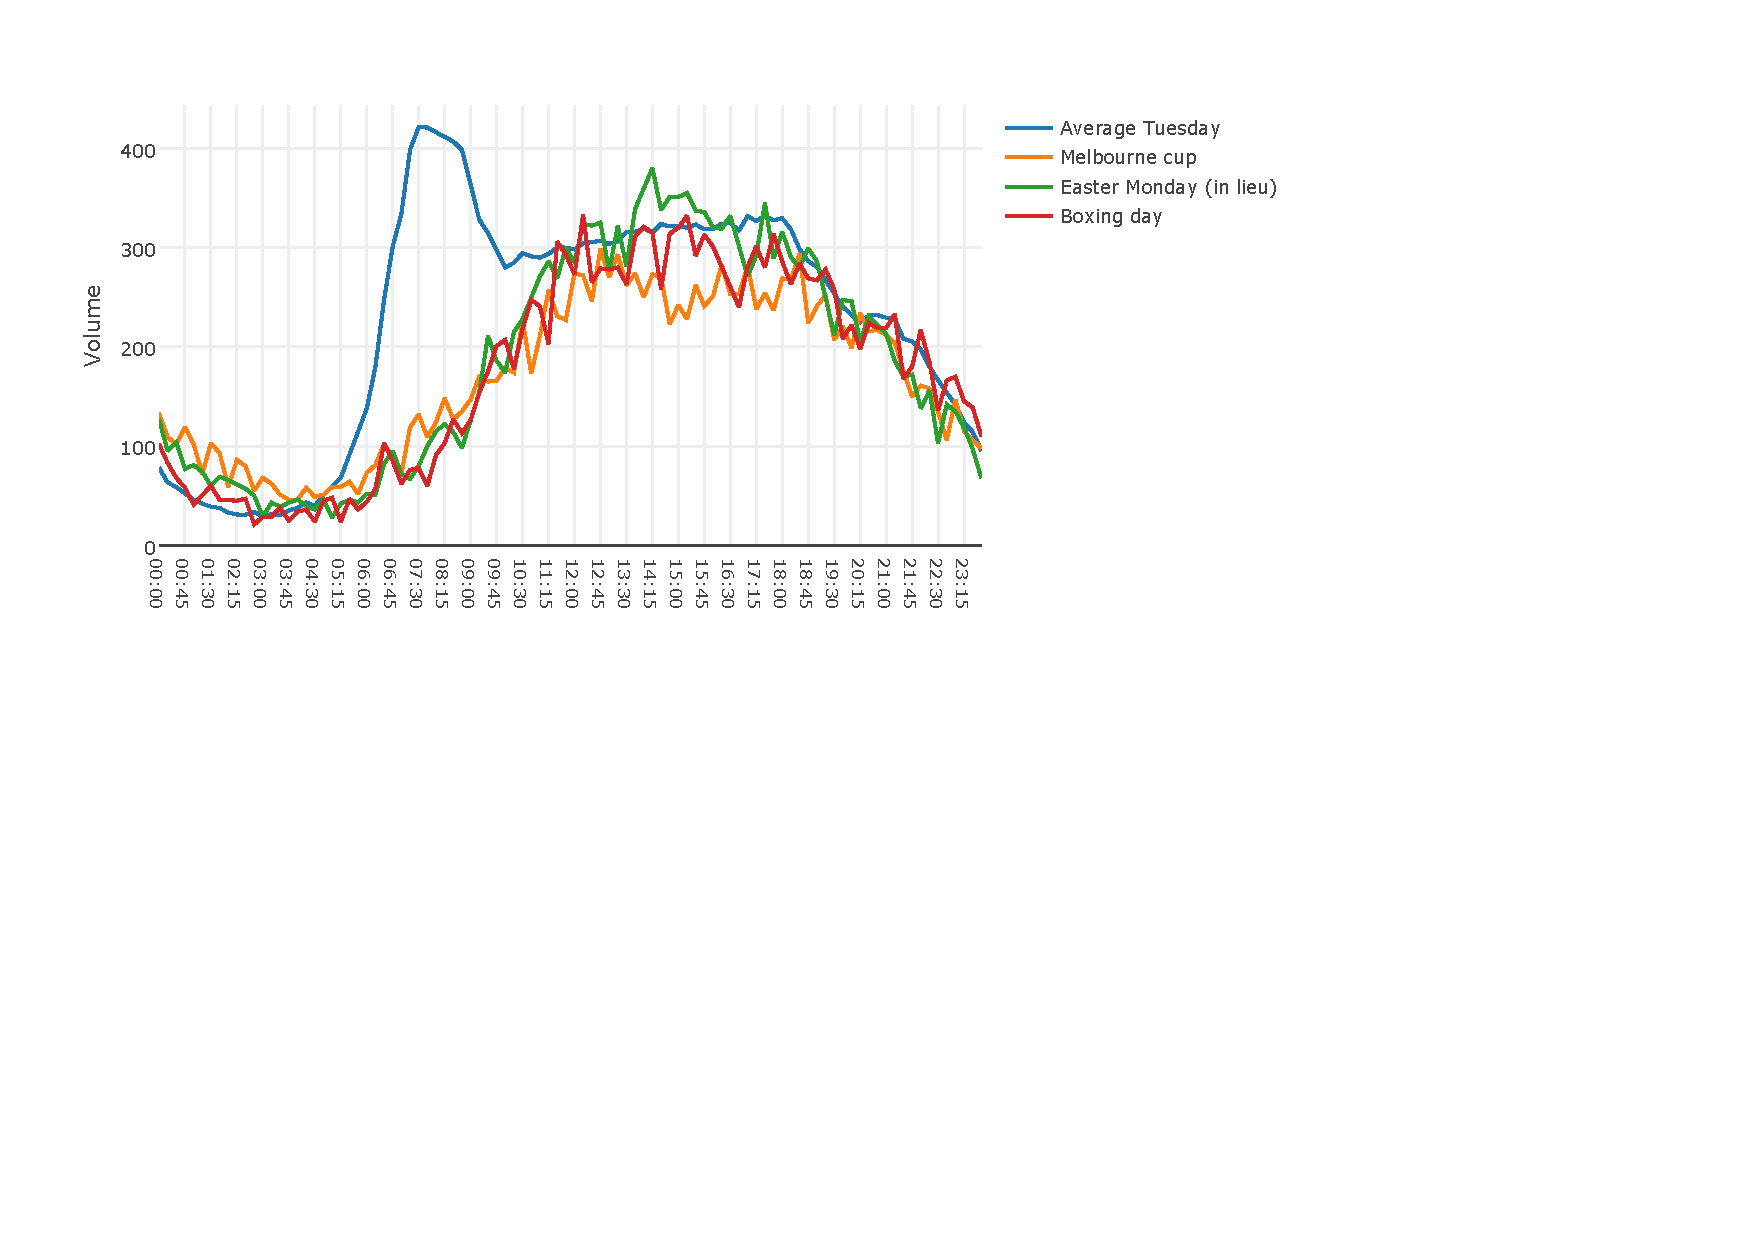
\includegraphics[width=0.4\textwidth]{Plots/holiday-tuesdays.pdf}
    \label{fig:HolidayTuesdays}}

    \subfloat[Wednesdays][Wednesdays]{
    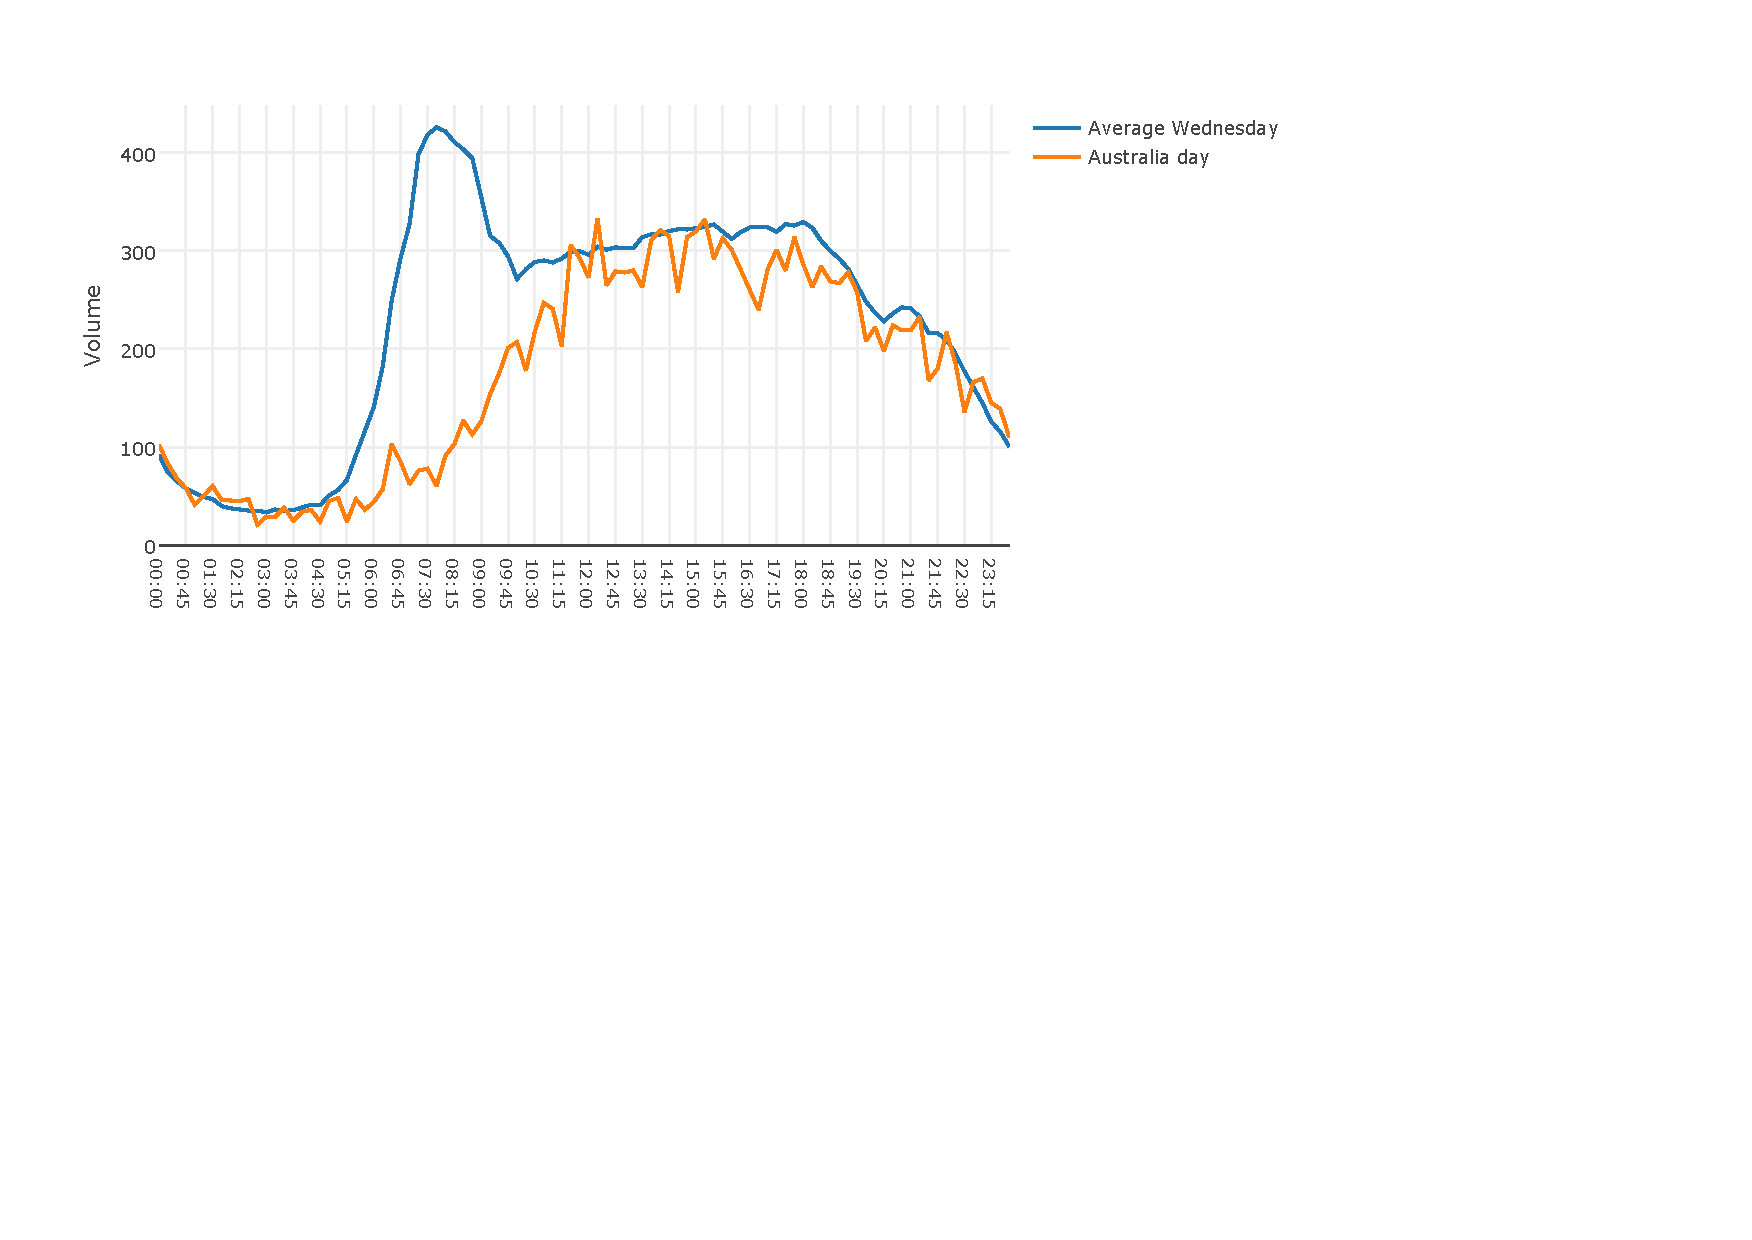
\includegraphics[width=0.4\textwidth]{Plots/holiday-wednesdays.pdf}
    \label{fig:HolidayWednesdays}}
    \qquad
    \subfloat[Thursdays][Thursdays]{
    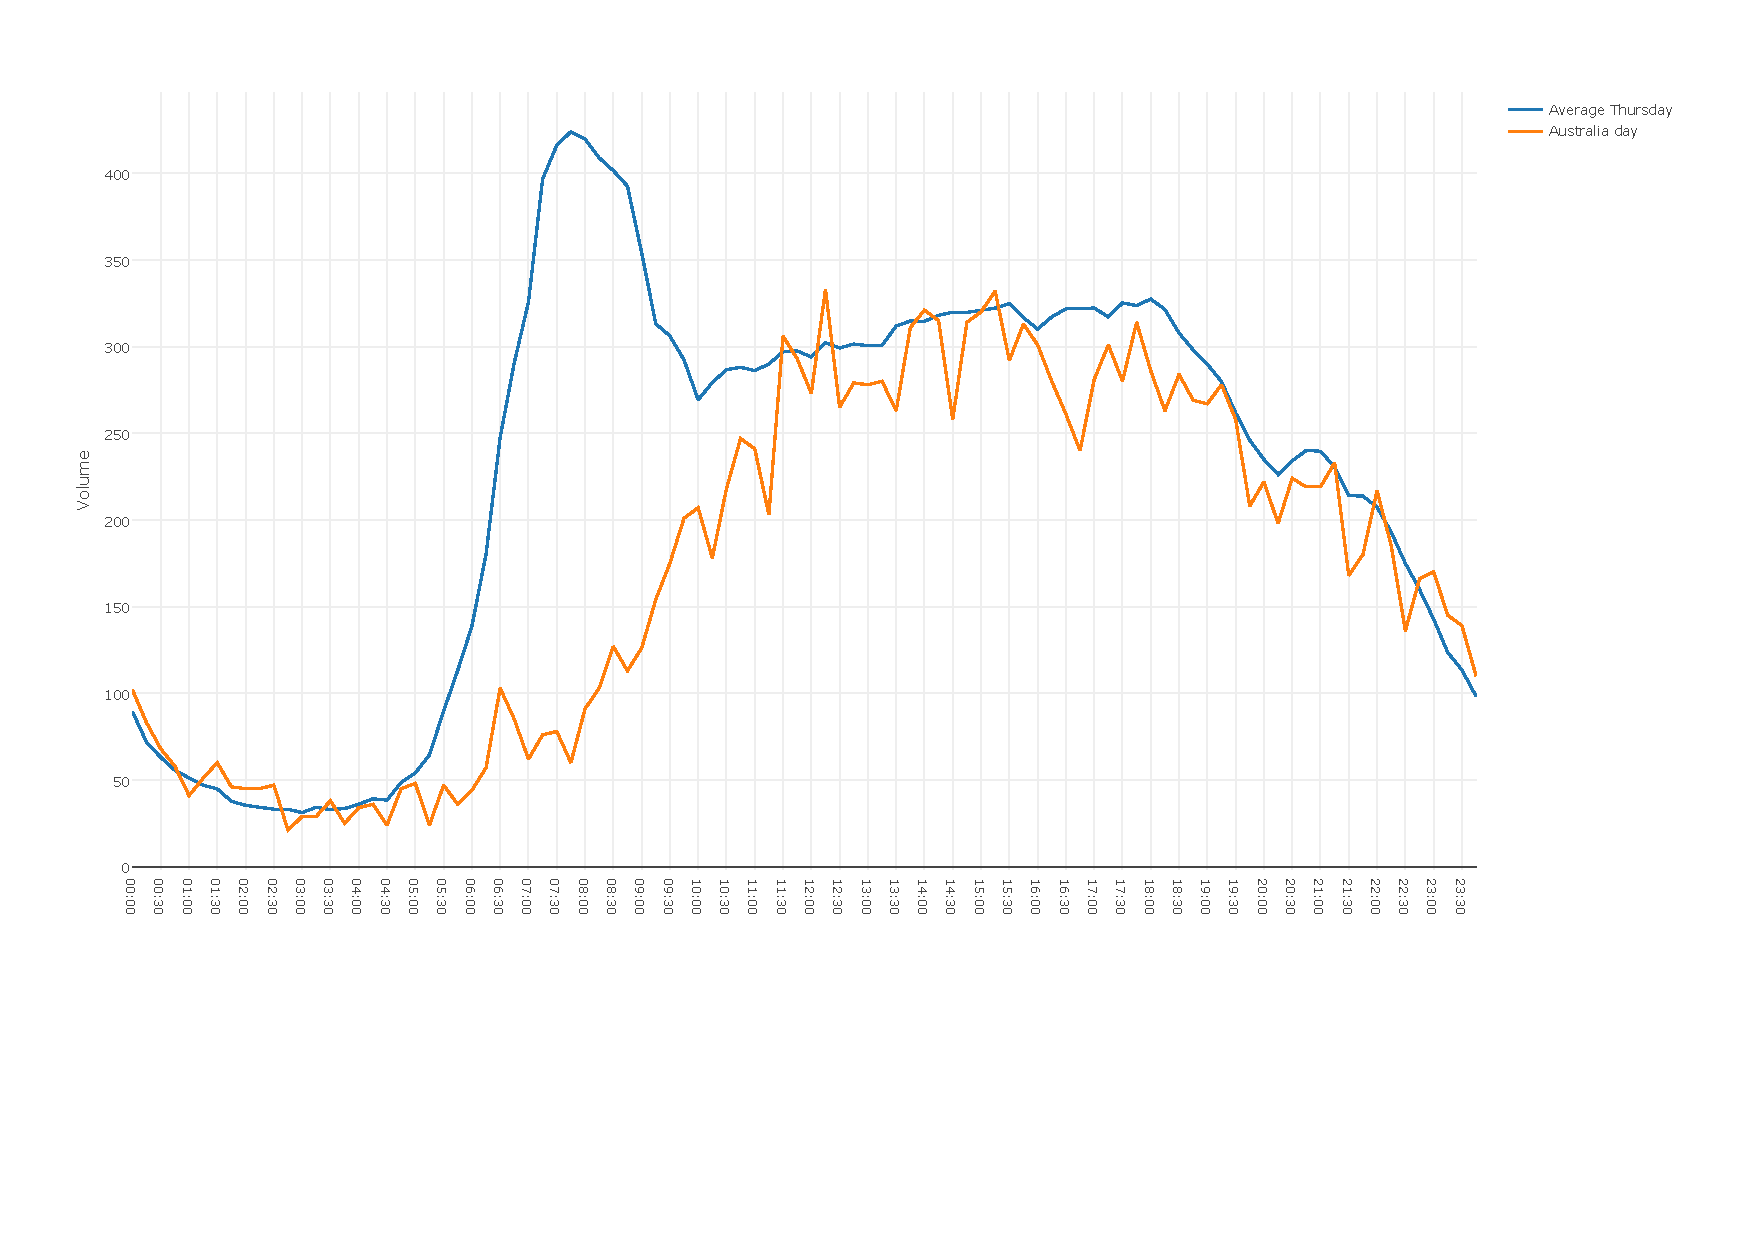
\includegraphics[width=0.4\textwidth]{Plots/holiday-thursdays.pdf}
    \label{fig:HolidayThursdays}}

    \subfloat[Fridays][Fridays]{
    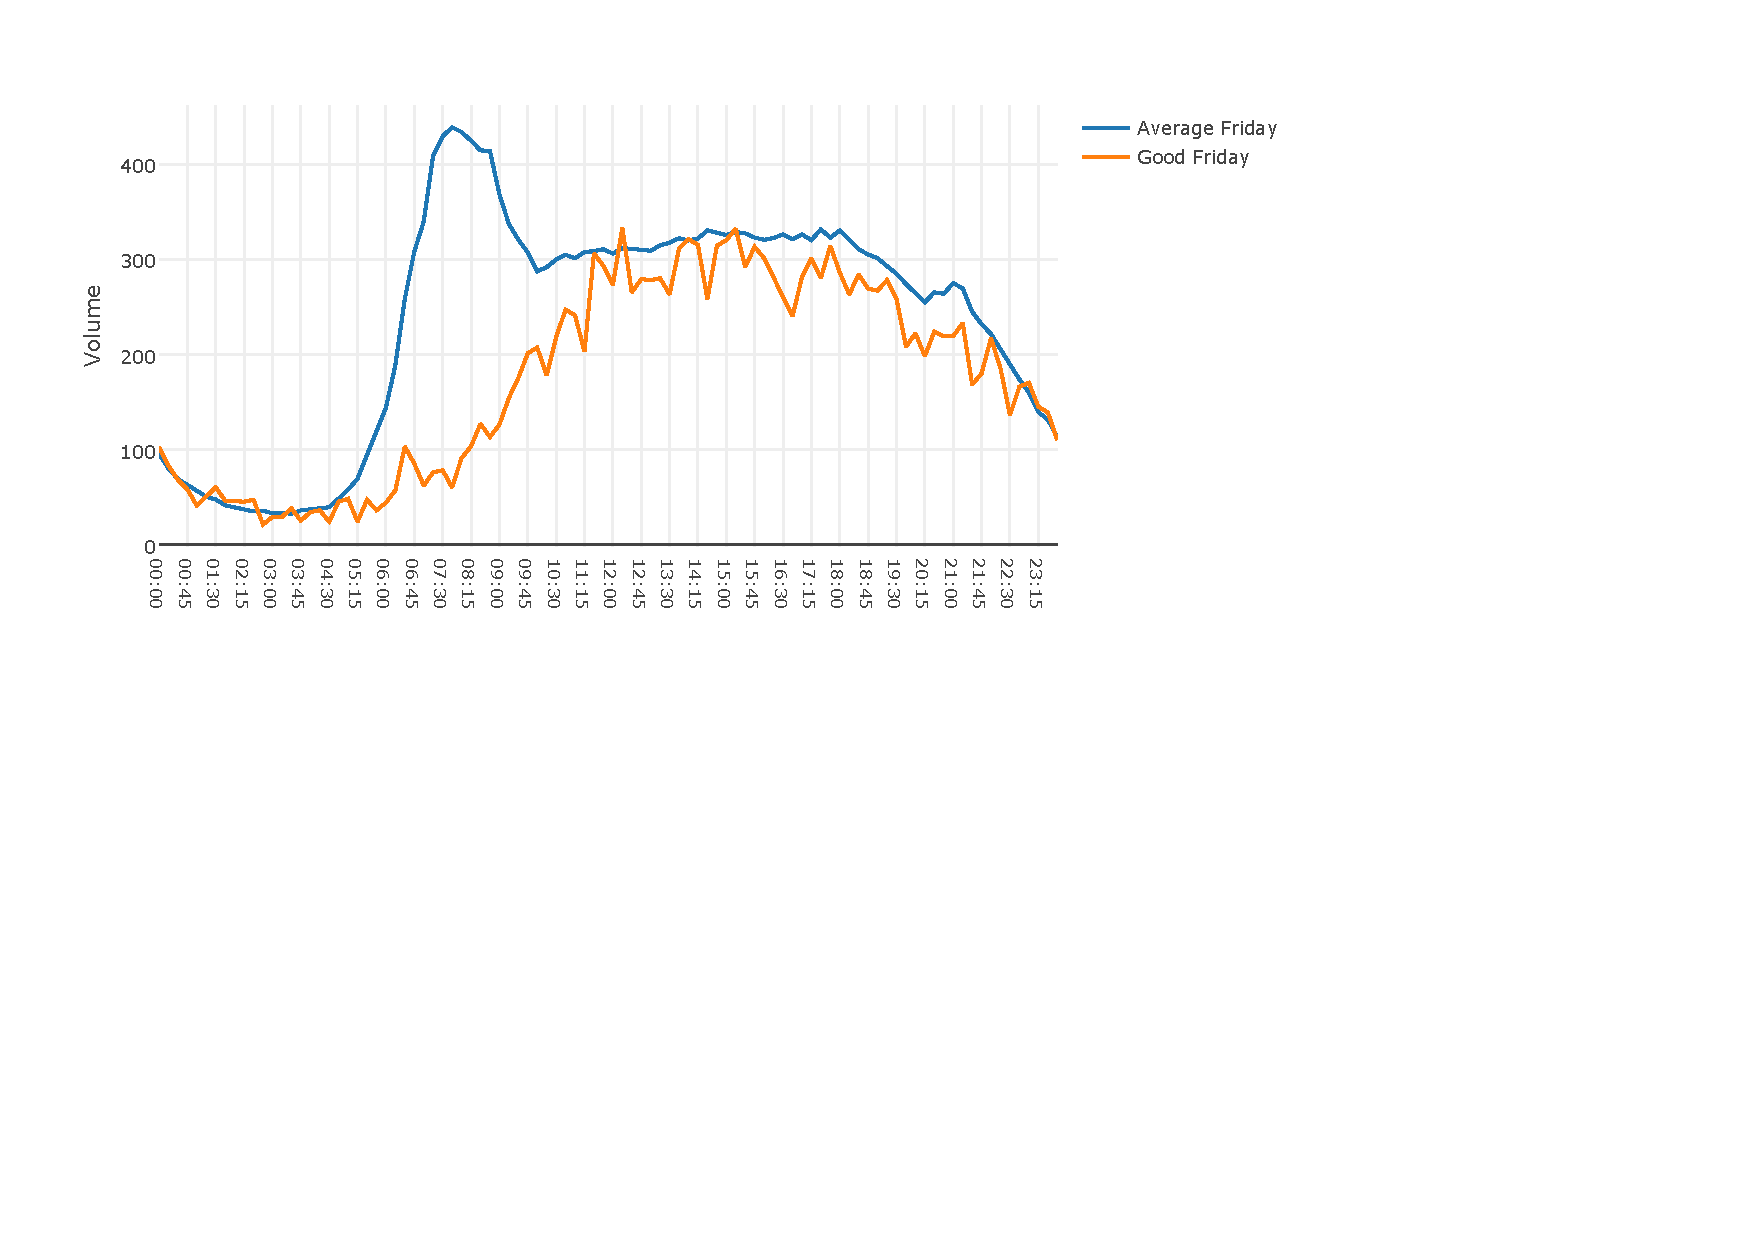
\includegraphics[width=0.4\textwidth]{Plots/holiday-fridays.pdf}
    \label{fig:HolidayFridays}}

    \caption[Impact of public holidays on traffic volume]{Variations in traffic volume caused by
     public holidays}
   \label{fig:Holidays}
\end{figure}

\subsection{Secular trends}
The secular variations in traffic volume data is important from infrastructre planning point of
view. While long term foracasting of traffic data is out of the scope for this work it is interesting
to find out the trends in the traffic volume, to see how it has evolved over the years.
Figure \ref{fig:AverageTrafficVolume} shows the average daily, weekly, monthly and yearly traffic
volume.

\begin{figure}[h]
    \centering
    \subfloat[Daily][Daily]{
    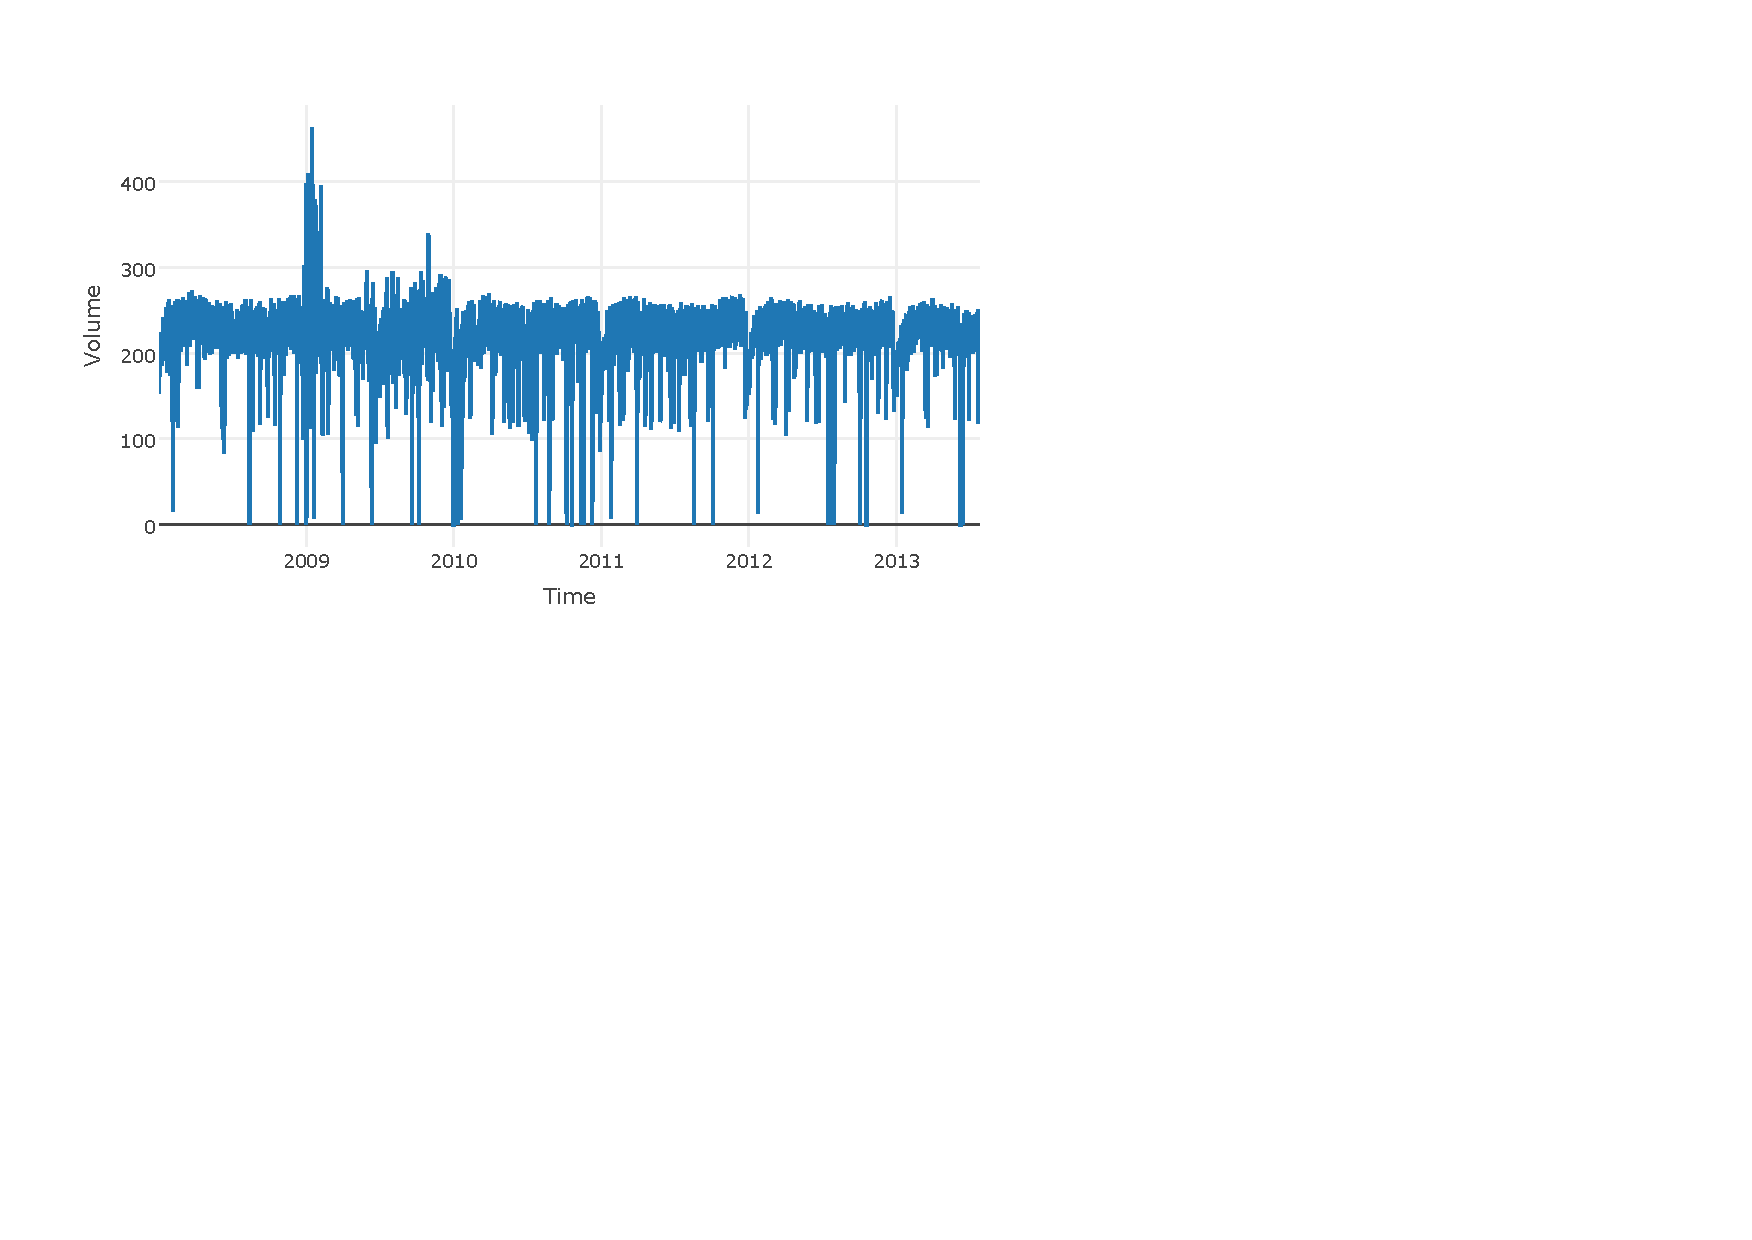
\includegraphics[width=0.4\textwidth]{Plots/averages-daily.pdf}
    \label{fig:AverageDaily}}
    \qquad
    \subfloat[Weekly][Weekly]{
    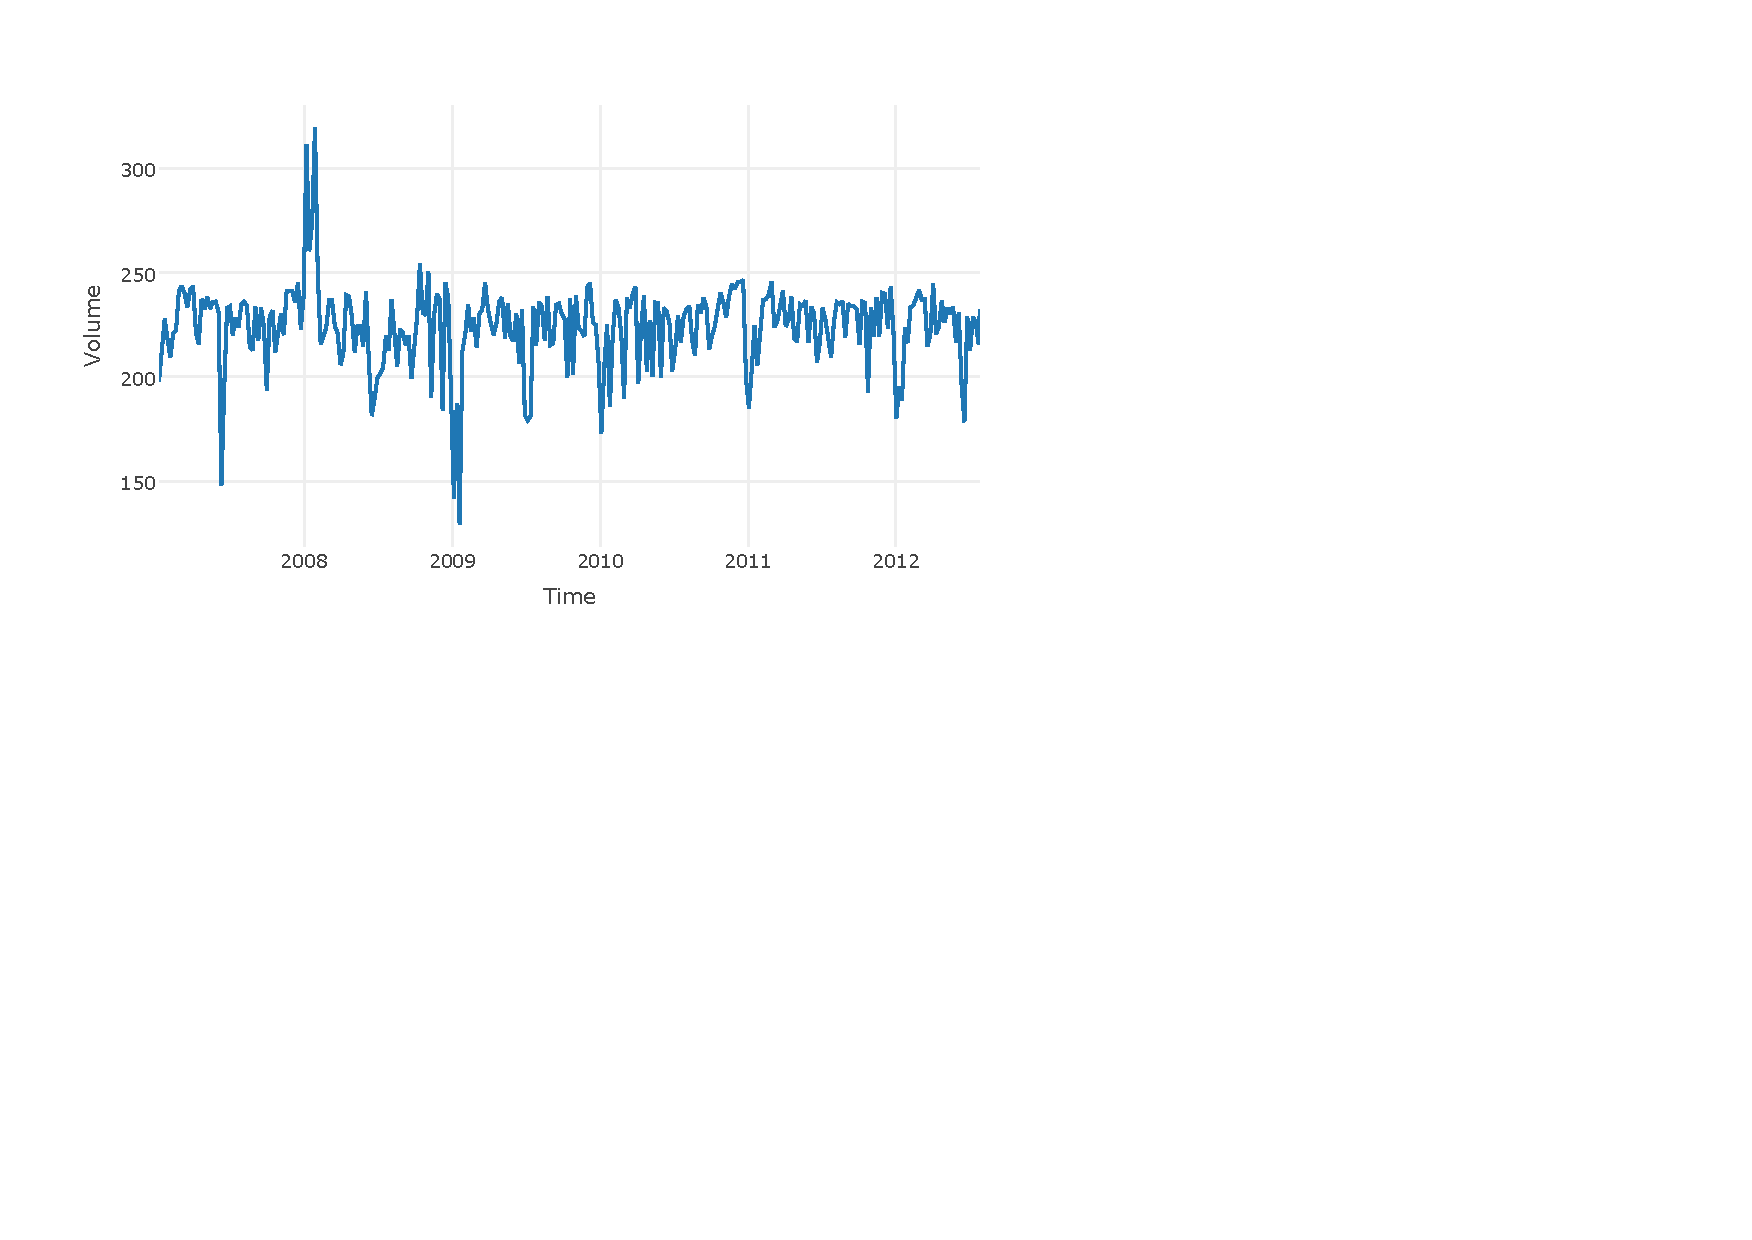
\includegraphics[width=0.4\textwidth]{Plots/averages-weekly.pdf}
    \label{fig:AverageWeekly}}

    \subfloat[Monthly][Monthly]{
    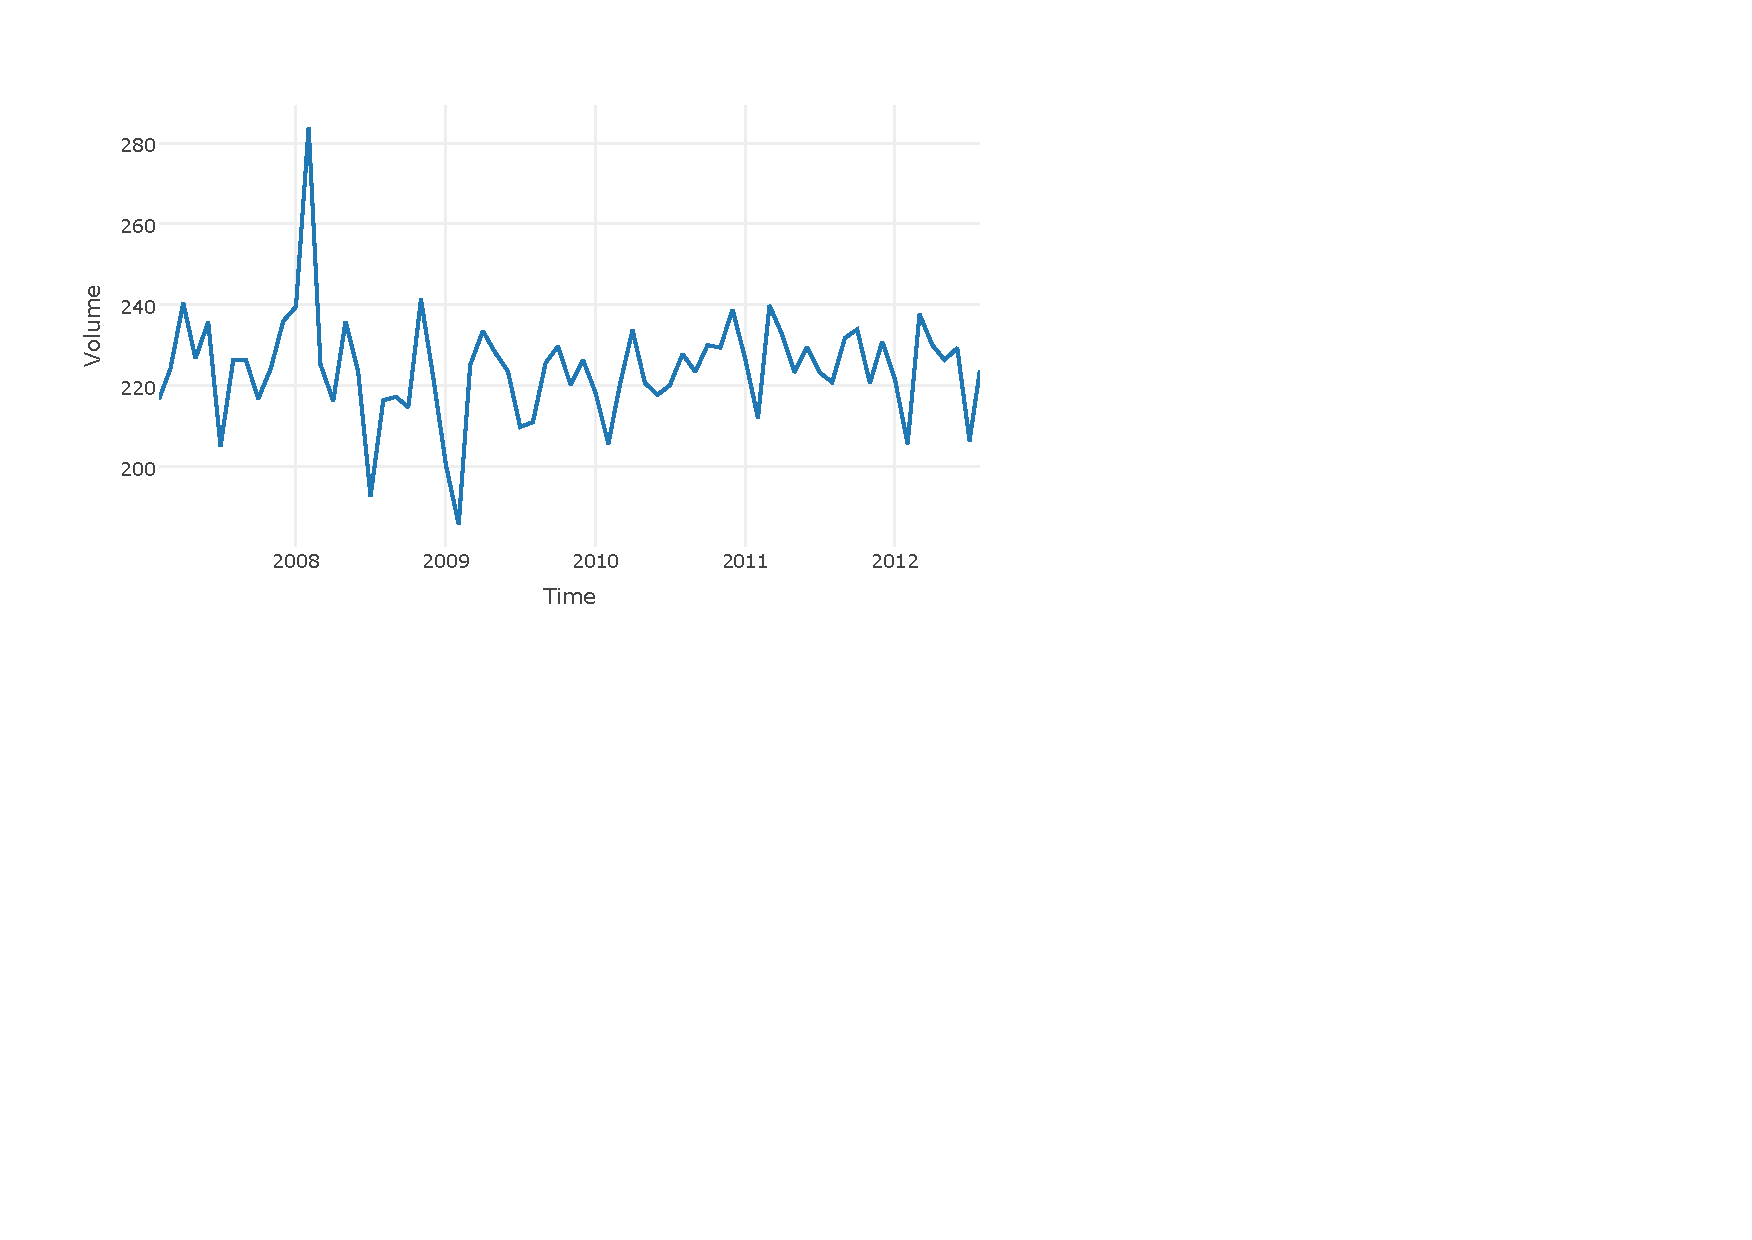
\includegraphics[width=0.4\textwidth]{Plots/averages-monthly.pdf}
    \label{fig:AverageMonthly}}
    \qquad
    \subfloat[Yearly][Yearly]{
    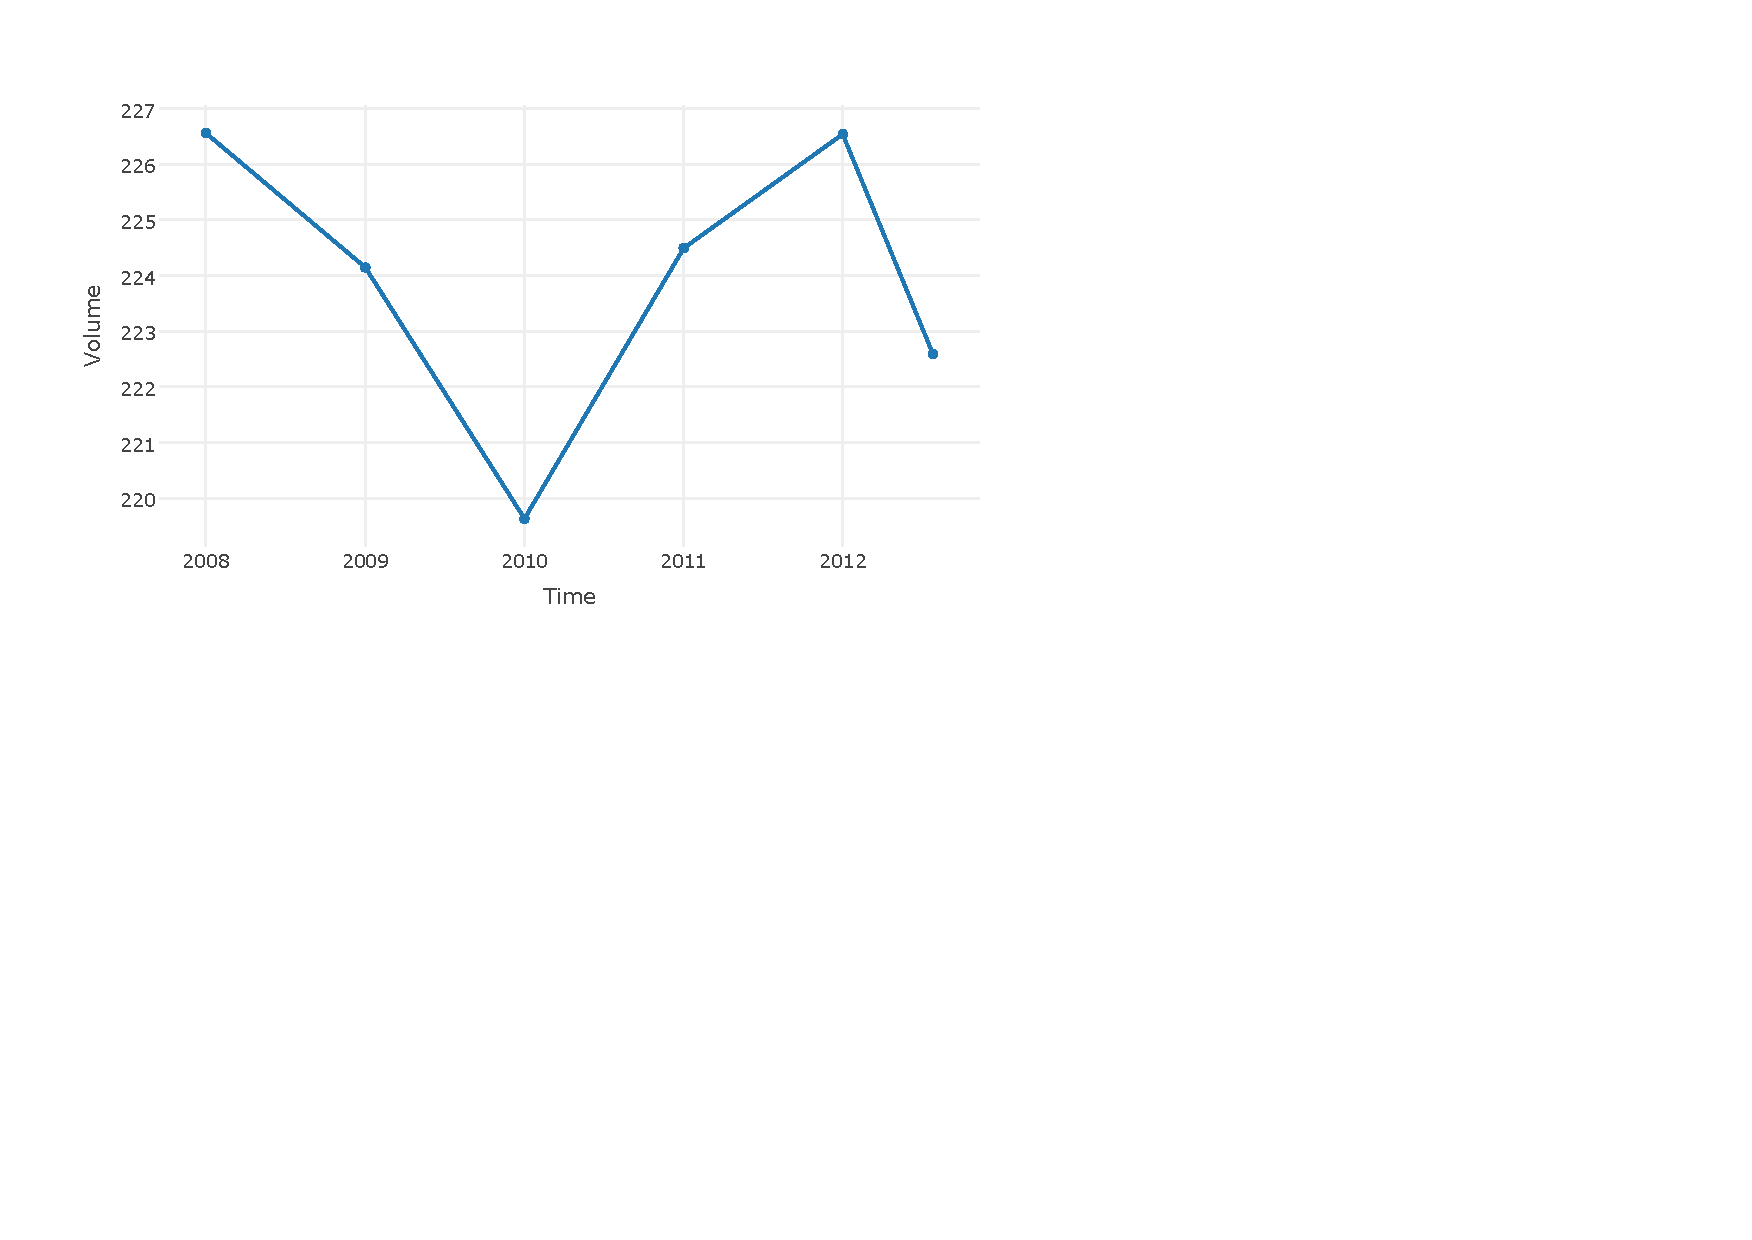
\includegraphics[width=0.4\textwidth]{Plots/averages-yearly.pdf}
    \label{fig:AverageYearly}}

    \caption[Average Traffic Volume]{(a) daily, (b) weekly, (c) monthly and (d) yearly average of
    traffic volume (15 mins interval) at a site location from the period 01/01/2008 to 26/07/2013}
   \label{fig:AverageTrafficVolume}
\end{figure}
